\documentclass{article}
\usepackage[T1]{fontenc}
\usepackage{geometry}
\usepackage{booktabs}
\usepackage{longtable}
\usepackage{array}
\usepackage{graphicx}
\usepackage{svg}
\usepackage{xcolor}
\usepackage{titling}
\usepackage{fancyhdr}
\usepackage{tocloft}
\usepackage{lastpage}
\usepackage{float}  % Required for [H] figure placement
\usepackage{tikz}   % Required for QUPER diagrams
\usepackage{pgfplots}
\pgfplotsset{compat=1.18}
\usepackage{pgf-pie}
\usepackage{amssymb}  % Required for \square checkbox symbol
\usepackage{eurosym}  % Required for \euro symbol
\geometry{a4paper, margin=1in}
\setlength{\headheight}{23pt}  % Fix header height warning
% Table of contents formatting
\renewcommand{\cftsecleader}{\cftdotfill{\cftdotsep}}
\setcounter{tocdepth}{2} % Show up to subsections only
\setlength{\cftbeforesecskip}{0.3cm}
\begin{document}
% Custom Title Page
\begin{titlepage}
    \centering
    
    % University Logo
    \vspace*{1cm}
    \includegraphics[width=0.3\textwidth]{images/bth_logo.png}
    
    \vspace{1.5cm}
    
    % Project Name - PROMINENT
    {\Huge\bfseries CookWise\par}
    
    \vspace{0.8cm}
    
    % Document Type
    {\LARGE System Requirements Document\par}
    
    \vspace{1cm}
    
    % Course and Group Info
    {\large Group 03\par}
    \vspace{0.3cm}
    {\large PA2591 HT25 lp2\par}
    {\large Requirements Engineering and Product Management\par}
    
    \vspace{1cm}
    
    % Version Info
    \begin{tabular}{ll}
        \textbf{VERSION:} & 3 \\
        \textbf{REVISION DATE:} & 10/01/2026 \\
    \end{tabular}
    
    \vspace{1.5cm}
    
    % Project Supervisor
    \textbf{Project Supervisor:} Bhuwan Paudel
    
    \vspace{1cm}
    
    % Team Members Table
    \textbf{Team Members:}
    
    \vspace{0.5cm}
    
    \begin{tabular}{|l|l|}
        \hline
        \textbf{Name} & \textbf{Role} \\
        \hline
        Md Asif Iqbal Ahmed & Project manager \\
        \hline
        Letian Zhou & Customer coordinator \\
        \hline
        Runlin Long & Project member \\
        \hline
        Oghenero Jeremi Adjaino & Project member \\
        \hline
    \end{tabular}
    
    \vfill
    
\end{titlepage}
% Setup page style for table of contents and document
\pagestyle{fancy}
\fancyhf{} % Clear all headers and footers
\fancyhead[L]{CookWise\\Document}
\fancyhead[R]{System Requirements\\\textit{Version 3 - 10/01/2026}}
\fancyfoot[C]{Page \thepage\ of \pageref{LastPage}}
\renewcommand{\headrulewidth}{0.4pt}
\renewcommand{\footrulewidth}{0.4pt}
% Table of Contents
\tableofcontents
\thispagestyle{fancy}
\newpage
% Include all sections
\section{Introduction}

\subsection{Purpose and scope}

This document specifies the requirements for CookWise, a meal planning and grocery shopping optimization tool designed for the Swedish market. CookWise helps users plan their meals and optimize their grocery shopping by suggesting recipes based on current sales and promotions at major Swedish grocery stores such as ICA, Willys, and Coop.

\vspace{0.5cm}

\textbf{What the System Will Do}

CookWise will provide the following core capabilities:

\begin{itemize}
    \item Suggest recipes based on items that are currently on sale at local grocery stores (ICA, Willys, Coop)
    \item Allow users to search for recipes by specific ingredients
    \item Allow users to filter recipes by cuisine type, dietary restrictions, budget, and cooking time
    \item Display detailed recipe information including ingredients, quantities, cooking instructions, and nutritional data
    \item Enable users to rate and provide feedback on recipes
    \item Generate shopping lists automatically from selected recipes
    \item Show estimated cost savings by comparing regular prices versus sale prices across different stores
    \item Provide a map view showing store locations, price comparisons, and navigation routes for the shopping list
    \item Enable users to create accounts and save favorite recipes for future reference
\end{itemize}

\vspace{0.5cm}

\textbf{Benefits of the Product}

CookWise delivers several key benefits to users:

\begin{itemize}
    \item \textbf{Cost Savings:} Users can reduce grocery expenses by taking advantage of current sales and promotions when planning meals

    \item \textbf{Meal Variety:} Users discover new recipes and expand their cooking repertoire while staying within budget through intelligent sale based recipe recommendations

    \item \textbf{Informed Store Selection:} The system provides transparent price comparisons and store recommendations through a single platform, eliminating the need to manually check multiple store websites while enabling data driven shopping choices

    \item \textbf{Time Efficiency:} The system eliminates the need to manually browse multiple store flyers and match sales to recipes, significantly reducing weekly planning time

    \item \textbf{Reduced Food Waste:} By providing exact ingredient quantities and utilizing items on sale, the system helps minimize food waste at the household level
\end{itemize}

\vspace{0.5cm}

\textbf{System Goals}

The primary goals of CookWise are detailed in Section 1.4 as formal goal level requirements, covering cost effectiveness, meal variety through sale based recipe discovery, informed store selection, time efficiency, and waste reduction.

\vspace{0.5cm}

\textbf{What the System Will NOT Do}

To clarify the boundaries and scope of this project, CookWise will explicitly NOT include:

\begin{itemize}
    \item Processing of actual purchases or payment transactions
    \item Real time inventory tracking or stock availability at physical stores
    \item Home delivery, delivery scheduling, meal kit assembly, or courier services
    \item Creation of fully custom or AI generated personalized recipes without human review
    \item Nutritional consultation or medical dietary advice
\end{itemize}

\subsection{Definitions, acronyms, and abbreviations}

This section provides definitions of all terms, acronyms, abbreviations, and domain specific terminology used throughout this document.

\vspace{0.3cm}

\textbf{Requirement Identifiers}

Requirements in this document are identified using the following prefixes:

\begin{itemize}
    \item \textbf{DL}: Domain Level Requirement (e.g., DL1, DL2, DL3, DL4, DL5, DL6)
    \item \textbf{PR}: Product Requirement (e.g., PR1, PR2, PR3, ..., PR14)
    \item \textbf{DR}: Data Requirement (e.g., DR1, DR2, DR3, DR4)
    \item \textbf{QR}: Quality Requirement (e.g., QR1, QR2, QR3, QR4, QR5)
\end{itemize}

\vspace{0.3cm}

\textbf{Terms and Definitions}

\begin{longtable}{|p{4cm}|p{10cm}|}
\hline
\textbf{Term} & \textbf{Definition} \\
\hline
\endfirsthead
\hline
\textbf{Term} & \textbf{Definition} \\
\hline
\endhead
ACID Properties & A set of properties that guarantee reliable database transactions: Atomicity (transactions complete fully or not at all), Consistency (database remains in a valid state), Isolation (concurrent transactions don't interfere), and Durability (committed transactions persist permanently). \\
\hline
API & Application Programming Interface. A set of rules and protocols that allow different software applications to communicate with each other. \\
\hline
Consolidated Shopping List & A shopping list that combines ingredients from multiple selected recipes, aggregating quantities for items that appear in more than one recipe. \\
\hline
CookWise & The name of the meal planning and grocery shopping optimization system described in this document. The product is designed for the Swedish market. \\
\hline
GDPR & General Data Protection Regulation. A comprehensive data privacy and security law in the European Union (EU 2016/679) that mandates how the system must handle and protect personal data of users. \\
\hline
Recipe & A structured set of instructions for preparing a dish, including a list of ingredients with quantities, step by step cooking instructions, preparation time, and nutritional information. \\
\hline
Sale Item & A product that is currently offered at a discounted price or promotional price by a grocery retailer. Sale items are the basis for recipe suggestions in CookWise. \\
\hline
Shopping List & An automatically generated list of ingredients required for selected recipes, organized by product category and store, with quantities and estimated prices. \\
\hline
Stakeholder & Any individual, group, or organization that has an interest in or is affected by the CookWise system. Stakeholders include end users, grocery retailers, development team members, and regulatory bodies. \\
\hline
Total Basket Price & The sum of all ingredient prices for a complete shopping list at a specific store, including all applicable promotions and discounts. This value is used to compare the cost-effectiveness of shopping at different stores for the same set of ingredients or equivalent items. \\
\hline
Web Scraping & An automated technique for extracting data from websites by parsing HTML content. CookWise uses web scraping to collect product prices, sale information, and store locations from retailer websites on a daily basis. \\
\hline
\end{longtable}

\subsection{Overview}

This document is structured to systematically present the requirements for the CookWise system, from initial stakeholder analysis through detailed specifications to a phased release plan. The organization of subsequent sections is as follows:

\vspace{0.3cm}

\textbf{Section 2: Stakeholder Identification and Analysis} identifies all individuals, groups, and organizations with an interest in the CookWise system. It analyzes their roles, influence levels, expectations, and potential impact on the project. This section establishes who the system must satisfy and whose needs must be balanced during development.

\vspace{0.3cm}

\textbf{Section 3: Requirements Elicitation Techniques} describes the specific methods used to gather requirements from stakeholders identified in Section 2. Five techniques are employed: brainstorming sessions, semi structured interviews, requirements workshops, questionnaires, and prototyping. Each technique's purpose, execution process, and key findings are documented.

\vspace{0.3cm}

\textbf{Section 4: System Requirements} forms the core of this document, detailing all requirements for CookWise. This section is subdivided into four parts:

\begin{itemize}
    \item \textbf{Section 4.1: Domain Requirements} describes high level business rules and constraints inherent to the grocery shopping and meal planning domain that the system must respect.
    
    \item \textbf{Section 4.2: Product Requirements} specifies the concrete functional behaviors and capabilities the system must provide to users.
    
    \item \textbf{Section 4.3: Data Requirements} defines the data entities (such as users, recipes, products, stores), their attributes, and the relationships between them that the system must manage. An Entity Relationship Diagram (ERD) is included.
    
    \item \textbf{Section 4.4: Quality Requirements} elaborates on non functional requirements using the QUPER model. Five quality aspects are specified in detail: accuracy, reliability, performance, usability, and scalability.
\end{itemize}

\vspace{0.3cm}

\textbf{Section 5: Requirements Prioritization} presents the prioritization of all requirements from Section 4 using three complementary techniques: the 100 Dollar Test (ratio scale prioritization), ranking (ordinal scale prioritization), and Numerical Assignment (ordinal scale prioritization). The results guide development sequencing and resource allocation.

\vspace{0.3cm}

\textbf{Section 6: Release Planning} proposes a phased delivery strategy based on the prioritized requirements. Requirements are grouped into two major releases, each consisting of three two week sprints. Dependencies between requirements and risk factors are considered in the release plan.

\vspace{0.3cm}

\textbf{Section 7: Policy and Regulation Requirements} lists all legal, regulatory, and compliance requirements that CookWise must adhere to. This includes GDPR compliance, consumer protection laws, food information regulations, accessibility standards, and Swedish national legislation.

\vspace{0.3cm}

\textbf{Section 8: References} provides a comprehensive list of all cited documents, academic sources, standards, legal texts, and technical documentation referenced throughout this Software Requirements Document.

\vspace{0.3cm}

\textbf{Section 9: Document Revision History} tracks all versions of this document, including dates, version numbers, and descriptions of changes made in each revision.

\vspace{0.3cm}

\textbf{Section 10: Appendices} contains supplementary materials including the questionnaire, the PlantUML source code for diagrams, the AI-generated prototype prompt, and other supporting documentation.

\vspace{0.3cm}

This structure ensures a logical progression from understanding stakeholders and gathering their needs, to formally specifying requirements, prioritizing them, and planning their implementation in releases.

\subsection{Goals of the Product (Goal Level Requirements)}

This section describes the high level business goals and strategic objectives that CookWise aims to achieve.

\vspace{0.5cm}

\textbf{Goal\_1: Increase Grocery Cost Effectiveness}

Users shall be able to reduce their grocery shopping expenses by leveraging sale items and promotions when planning meals.

\vspace{0.5cm}

\textbf{Goal\_2: Expand Meal Variety and Recipe Discovery}

Users shall discover new recipes and expand their cooking repertoire while staying within their budget constraints through intelligent recipe recommendations based on current sales and promotions.

\vspace{0.5cm}

\textbf{Goal\_3: Optimize Store Selection}

Users shall be able to identify the most cost effective grocery store for their shopping needs based on total basket price and proximity to their location.

\vspace{0.5cm}

\textbf{Goal\_4: Reduce Shopping Planning Time}

Users shall spend significantly less time on meal planning and shopping list preparation compared to manual browsing of multiple store flyers and recipe websites.

\vspace{0.5cm}

\textbf{Goal\_5: Reduce Food Waste and Environmental Impact}

Users shall reduce food waste at the household level through accurate ingredient quantities and strategic meal planning, contributing to environmental sustainability.

\subsection{Context diagram for the system}

The context diagram in Figure \ref{fig:context_diagram} illustrates the CookWise system and its interactions with external entities. The CookWise Main System (shown in blue) is the central component that processes user inputs and provides recipe recommendations, shopping lists, and store price comparisons.

External entities include:

\begin{itemize}
    \item \textbf{Users}: Primary actors who provide preferences and location, receiving recipe suggestions and shopping lists.

    \item \textbf{Supermarket Websites}: Data sources (ICA, Willys, Coop) providing product prices, sale data, and store locations via web scraping.

    \item \textbf{Maps and Geolocation Service}: External service (Google Maps) providing store coordinates and navigation.

    \item \textbf{AI Recipe Generation Service}: External AI service (OpenAI/Claude) generating recipe suggestions based on sale items and user preferences.

    \item \textbf{External Authentication Service}: Third party authentication providers (Google and Apple) handling user login and account creation.
\end{itemize}

The diagram shows data flows between CookWise and external entities, with arrows indicating direction of information exchange.

\begin{figure}[H]
    \centering
    \includegraphics[width=0.9\textwidth]{images/context_diagram.png}
    \caption{Context Diagram for CookWise System}
    \label{fig:context_diagram}
\end{figure}
\section{Stakeholder Identification and Analysis}

The following stakeholders have been identified for the system. For each stakeholder, we describe who they are, what goals they have for the system, why they would use or support it, and what concerns or risks they see. They are organized into four categories based on their relationship to the product.

\subsection{Daily Users}

These are the end users who will interact with the application regularly.

\begin{longtable}{|p{4cm}|p{8cm}|p{2cm}|}
\hline
\textbf{Stakeholder} & \textbf{Description} & \textbf{Priority} \\
\hline
\endfirsthead
\hline
\textbf{Stakeholder} & \textbf{Description} & \textbf{Priority} \\
\hline
\endhead
Budget Conscious Home Cooks & Families and individuals who do household grocery shopping and are highly price sensitive. They want the system to help them discover recipes based on current store sales, calculate their total savings, and reduce food waste by providing exact ingredient amounts. However, they worry that the system might recommend cheap items that do not match their preferences. They are concerned about the time needed to learn the system. & Critical \\
\hline
Time Constrained Users & Busy professionals, young workers, and people who recently moved to Sweden. These users have limited time for meal planning and grocery shopping. They need quick recipe ideas, efficient shopping routes, and help finding local stores. Their main worry is whether the app will be easy to use or add complexity to their schedules. & Critical \\
\hline
Culinary Enthusiasts & People who love cooking and enjoy trying new recipes and cuisines. They want the system to suggest creative recipes using seasonal ingredients or discounted specialty items. This helps them explore new dishes while keeping costs reasonable. They are concerned that the system might not provide enough variety beyond basic recipes. & High \\
\hline
\end{longtable}

\subsection{Internal Team (Development and Management)}

These are team members within our organization who are responsible for building and managing the product.

\begin{longtable}{|p{4cm}|p{8cm}|p{2cm}|}
\hline
\textbf{Stakeholder} & \textbf{Description} & \textbf{Priority} \\
\hline
\endfirsthead
\hline
\textbf{Stakeholder} & \textbf{Description} & \textbf{Priority} \\
\hline
\endhead
Product Manager & The person who owns the product vision and decides which features are most important. They gather user feedback, study the market, and ensure the product achieves business success. They must balance what different stakeholders want and make smart decisions about what to build and when. Their main concern is ensuring the product provides real value to users while remaining technically and financially feasible. & Critical \\
\hline
Development Team & The technical staff who design, build, test, and maintain the system. They need clear requirements that explain exactly what to build. They must ensure the system works reliably. Their concerns include handling technical challenges, connecting multiple external services such as AI for recipes and maps for locations, and ensuring the system performs well when many users access it simultaneously. & Critical \\
\hline
Marketing \& Sales Team & The team who promotes the application, acquires new users, and builds partnerships with grocery stores. They need strong messages that clearly explain why users should choose this app over others. Their success depends on securing data partnerships with stores and achieving user adoption targets. They worry about market competition and the difficulty of convincing stores to collaborate. & High \\
\hline
\end{longtable}

\subsection{Business Partners and Resource Providers}

External organizations provide essential data, services, or resources for the system.

\begin{longtable}{|p{4cm}|p{8cm}|p{2cm}|}
\hline
\textbf{Stakeholder} & \textbf{Description} & \textbf{Priority} \\
\hline
\endfirsthead
\hline
\textbf{Stakeholder} & \textbf{Description} & \textbf{Priority} \\
\hline
\endhead
Grocery Store Chains (ICA, Willys, Coop) & Swedish supermarket chains that provide pricing and product data through web scraping. In the future, there will be official partnerships where stores directly share their data. They benefit from increased customer traffic and faster turnover of expiring or seasonal products. Their concerns include data sharing agreements, competitive implications, and alignment with their own digital strategies. & Critical \\
\hline
AI Service Provider & An external company that provides artificial intelligence services through an API to generate and recommend recipes. The quality, speed, and cost of their service directly affects how well the recipe feature works. Their concerns include API usage costs at scale and maintaining reliable service availability. & High \\
\hline
Map \& Geolocation Service Provider & An external service such as Google Maps that provides location data, calculates distances between places, and suggests routes. This service is essential for helping users identify the closest and most convenient stores. Their concerns include usage costs, API rate limits, and compliance with their terms of service. & High \\
\hline
\end{longtable}

\subsection{Regulatory Compliance}

\textbf{Note on Regulatory Authorities:} Data protection authorities (such as GDPR enforcement agencies in the European Union) and other regulatory bodies are not explicitly listed as stakeholders in this document. Instead, their influence is captured through regulatory and compliance requirements embedded in Section 4 (Domain Level Requirements) and Section 7 (Policy and Regulation Requirements). Specifically, DL2 addresses GDPR compliance for user and partner data, ensuring the system meets all data protection obligations without treating regulatory bodies as direct stakeholders.
% Section 3: Requirements Elicitation Techniques
\section{Requirements Elicitation Techniques}

This section describes the elicitation techniques used to gather requirements for the CookWise system. We employed five different techniques to ensure comprehensive requirements coverage from multiple perspectives.

\subsection{Brainstorming}

\textbf{Selection Rationale:} Brainstorming was used to generate creative solution ideas through two strategic sessions: one before interviews to formulate questions, and one after interviews to develop solution ideas based on validated user pain points.

\vspace{0.5cm}

\textbf{Execution:}

\begin{itemize}
    \item \textbf{Participants:} All four team members (Project Manager, Customer Coordinator, two Project Members)
    \item \textbf{Session 1 - Pre-Interview (90 min):} Generated 18 hypothetical pain points to inform interview questions around: "What problems might budget-conscious families face when planning meals and shopping for groceries?"
    \item \textbf{Session 2 - Post-Interview (90 min):} Generated 23 feature ideas based on five key user insights from interviews. Ideas were captured on whiteboard following classic brainstorming principles (no criticism during generation, encouraging wild ideas, building on others' suggestions)
\end{itemize}

\textbf{Requirements Elicited:}

\begin{table}[h]
\centering
\caption{Requirements from Brainstorming}
\begin{tabular}{|l|l|}
\hline
\textbf{Requirement ID} & \textbf{Description} \\
\hline
PR2 & AI generated recipe recommendations using discounted ingredients \\
\hline
PR3 & Recipe filtering (cuisine, dietary restrictions, cooking time, difficulty) \\
\hline
PR4 & Automatic shopping list generation from selected recipes \\
\hline
PR8 & Store recommendation based on total cost and location \\
\hline
PR9 & Display detailed savings calculation \\
\hline
PR11 & Show additional ingredients needed, prioritizing sale items \\
\hline
PR13 & Store user preferences for items and recipes \\
\hline
QR1 & Performance: Fast recipe generation and page loading \\
\hline
QR2 & Usability: Easy first-time experience \\
\hline
\end{tabular}
\end{table}

\textbf{Key Insight:}

Comparing Session 1 hypotheses with interview findings revealed significant mismatches. The team initially assumed users wanted multi-store shopping optimization, but interviews showed strong preference for single-store convenience, validating the importance of user research before finalizing requirements.

\subsection{Interviews}

\textbf{Selection Rationale:} Semi-structured interviews were conducted early in the project to gain deep, qualitative understanding of users' grocery shopping journeys, pain points, and decision-making processes.

\vspace{0.4cm}

\textbf{Execution:}

\begin{itemize}
    \item \textbf{Participants:} 10 individuals in Karlskrona (5 university students, 2 professionals, 3 household members)
    \item \textbf{Duration:} 5-10 minutes per interview
    \item \textbf{Method:} Semi-structured, in-person interviews focusing on recent shopping experiences
    \item \textbf{Topics Covered:} Meal planning habits, store selection criteria, price comparison behaviors, recipe discovery
\end{itemize}

\textbf{Requirements Elicited:}

\begin{table}[h]
\centering
\caption{Requirements from Interviews}
\begin{tabular}{|l|l|}
\hline
\textbf{Requirement ID} & \textbf{Description} \\
\hline
\multicolumn{2}{|l|}{\textit{\textbf{Domain Requirements}}} \\
\hline
DL3 & Single store shopping constraint \\
\hline
DL4 & Include all applicable promotions in basket price \\
\hline
\multicolumn{2}{|l|}{\textit{\textbf{Product Requirements}}} \\
\hline
PR2 & AI recipe suggestions using discounted ingredients \\
\hline
PR8 & Store recommendation based on total cost and distance \\
\hline
PR9 & Display detailed savings breakdown \\
\hline
\multicolumn{2}{|l|}{\textit{\textbf{Quality Requirements}}} \\
\hline
QR1 & Performance critical (time savings valued) \\
\hline
QR3 & Reliability critical (price data accuracy) \\
\hline
\end{tabular}
\end{table}

\textbf{Key Insights:}

Interviews revealed two critical findings:

\begin{enumerate}
    \item Users strongly prefer single-store shopping despite being price-conscious, validating DL3 as a fundamental constraint.

    \item Time is valued more than money, with users spending 30+ minutes weekly manually matching sales to recipes, elevating QR1 (performance) to top priority.
\end{enumerate}

\subsection{Requirements Workshop}

\textbf{Selection Rationale:} A requirements workshop was conducted to consolidate findings from brainstorming and interviews into structured, traceable requirements including domain models, refined specifications, and traceability documentation.

\vspace{0.4cm}

\textbf{Execution:}

\begin{itemize}
    \item \textbf{Participants:} All four team members (Project Manager: Asif, Customer Coordinator: Letian Zhou, Project Members: Runlin, Oghenero)
    \item \textbf{Duration:} 4 hours in group room with large screen and whiteboard
    \item \textbf{Phase 1 - Domain Modeling (90 min):} Created Entity Relationship Diagram identifying core entities (User, Recipe, Ingredient, Store, Sale Item, Shopping List, Rating)
    \item \textbf{Phase 2 - Requirement Refinement (120 min):} Reviewed and refined all preliminary requirements for clarity, completeness, and traceability
    \item \textbf{Phase 3 - Traceability Mapping (30 min):} Linked requirements back to interview insights and business goals
\end{itemize}

\textbf{Requirements Elicited:}

\begin{table}[h]
\centering
\caption{Requirements Elicited from Workshop}
\begin{tabular}{|l|p{9cm}|}
\hline
\textbf{Req ID} & \textbf{Requirement Description} \\
\hline
\multicolumn{2}{|l|}{\textit{\textbf{Data Requirements (from ERD creation)}}} \\
\hline
DR1 & Core entity data models (User, Recipe, Ingredient, Rating, Store, Sale Item) \\
\hline
DR2 & Relationship models (Recipe-Ingredient, Shopping List, Shopping List Item) \\
\hline
DR3 & Data interchange formats (JSON for APIs, CSV/JSON for export, HTML parsing) \\
\hline
DR4 & System states (user sessions, operational states, recipe generation, shopping list) \\
\hline
\multicolumn{2}{|l|}{\textit{\textbf{Refined Product Requirements}}} \\
\hline
PR1 & External authentication (Google/Apple ID) \\
\hline
PR5 & User ratings and feedback for recipes (added during workshop discussion) \\
\hline
PR6 & Store AI generated recipes and their details \\
\hline
PR7 & Display complete recipe details with step by step instructions \\
\hline
PR10 & Search recipes by specific ingredients \\
\hline
PR12 & Daily web scraping to gather and update item data from store websites \\
\hline
PR14 & Display interactive map with store locations and navigation \\
\hline
PR15 & Calculate and display average ratings for recipes \\
\hline
\multicolumn{2}{|l|}{\textit{\textbf{Domain Requirements (refined)}}} \\
\hline
DL1 & Data sourced from store websites via web scraping (API partnerships future goal) \\
\hline
DL2 & Compliance with data protection regulations (GDPR) \\
\hline
DL5 & Rate limits and operational boundaries for external interfaces \\
\hline
DL6 & Domain events triggered by user actions and system operations \\
\hline
\end{tabular}
\end{table}

\textbf{Key Insights:}

\begin{enumerate}
    \item ERD creation revealed CookWise's value proposition depends on accurate, current sale price data, elevating QR3 (reliability/data accuracy) to top priority.

    \item The workshop confirmed DL3 (single store shopping) as a fundamental domain constraint, reflected in the ERD by linking each shopping list to exactly one store.

    \item Collaborative modeling revealed technical dependencies: PR1 (user accounts) must precede PR13 (preferences), and DL1 (sale data) plus DR1 (recipe database) must exist before PR2 (recipe suggestions) can function.
\end{enumerate}

\subsection{Questionnaire}

\textbf{Selection Rationale:} Questionnaires were used to obtain statistical evidence (n=25) for key assumptions identified during interviews, using primarily closed questions (multiple choice, Likert scales) to quantify findings such as single store shopping preference, time burden, and interest in CookWise.

\vspace{0.4cm}

\textbf{Execution:}

\begin{itemize}
    \item \textbf{Method:} Face-to-face questionnaire administered over a two week period
    \item \textbf{Locations:} BTH University campus and local gym in Karlskrona
    \item \textbf{Participants:} 25 individuals (12 university students, 3 professionals, 10 household members)
    \item \textbf{Questionnaire Design:} 15 questions (see Appendix A) organized into five sections: demographics, shopping behaviors, price sensitivity, meal planning habits, and interest in CookWise concept
    \item \textbf{Question Types:} Primarily closed questions (multiple choice, Likert scales 1-5) with limited open-ended questions
    \item \textbf{Duration:} 5-8 minutes per questionnaire
\end{itemize}

\textbf{Requirements Validated:}

The questionnaire provided quantitative validation for key requirements:

\begin{table}[h]
\centering
\caption{Requirements Validated Through Questionnaire}
\begin{tabular}{|l|p{9cm}|}
\hline
\textbf{Req ID} & \textbf{Validation Evidence} \\
\hline
\multicolumn{2}{|l|}{\textit{\textbf{Domain Requirements}}} \\
\hline
DL3 & Single store preference: 92\% always shop at one store, 8\% rarely visit multiple \\
\hline
\multicolumn{2}{|l|}{\textit{\textbf{Product Requirements}}} \\
\hline
PR2 & High interest in sale based recipe suggestions: 77\% rated 4 to 5 out of 5 \\
\hline
PR3 & Dietary filters important: 58\% indicated dietary restrictions or preferences \\
\hline
PR9 & Want to see savings details: 83\% said transparency in savings calculation is important \\
\hline
\multicolumn{2}{|l|}{\textit{\textbf{Quality Requirements}}} \\
\hline
QR1 & Time savings valued: 54\% spend 30+ minutes weekly on meal planning \\
\hline
QR2 & Usability important: Users want simple, intuitive interface \\
\hline
\end{tabular}
\end{table}

\vspace{0.2cm}

\textbf{Key Findings:}

\textbf{Finding 1: Time Burden Confirmed}

54\% of respondents spend 30+ minutes weekly on meal planning and grocery list preparation (mean: 37 minutes/week). This validates the system's focus on reducing planning time by 60 to 80\%.

\begin{figure}[H]
\centering
\begin{tikzpicture}
\begin{axis}[
    ybar,
    width=10cm,
    height=6cm,
    symbolic x coords={Less than 15min, 15-30min, 30-60min, More than 60min},
    xtick=data,
    x tick label style={font=\small, rotate=45, anchor=east},
    ylabel={Percentage of Respondents (\%)},
    ylabel style={font=\small},
    ymin=0, ymax=50,
    bar width=20pt,
    nodes near coords,
    every node near coord/.append style={font=\footnotesize},
]
\addplot coordinates {
    (Less than 15min,17) 
    (15-30min,29) 
    (30-60min,38) 
    (More than 60min,16)
};
\end{axis}
\end{tikzpicture}
\caption{Time Spent Weekly on Meal Planning and Grocery List Preparation}
\end{figure}

\textbf{Finding 2: Single Store Preference Validated}

92\% always shop at one store, 8\% rarely visit multiple stores (only in rare cases), and 0\% frequently shop at multiple stores. This strongly validates DL3 (single store constraint) as a fundamental requirement - virtually all users prefer single-store shopping, with no one regularly visiting multiple stores.

\begin{figure}[H]
\centering
\begin{tikzpicture}
\pie[
    text=legend,
    radius=2.5,
    color={green!60, yellow!60}
]
{92/Always one store, 8/Rarely multiple}
\end{tikzpicture}
\caption{Shopping Behavior: Single Store vs Multiple Stores}
\end{figure}

\textbf{Finding 3: High Interest in Sale Based Recipes}

When asked about interest in an app that automatically suggests recipes based on current sales, 77\% expressed high interest (rating 4 to 5 on a 5 point scale), with mean interest of 4.2/5.0. This validates PR2 (AI recipe suggestions based on sales) as a compelling core value proposition.

\begin{figure}[H]
\centering
\begin{tikzpicture}
\begin{axis}[
    ybar,
    width=10cm,
    height=6cm,
    symbolic x coords={Not interested (1-2), Neutral (3), Interested (4), Very interested (5)},
    xtick=data,
    x tick label style={font=\small, rotate=45, anchor=east},
    ylabel={Percentage of Respondents (\%)},
    ylabel style={font=\small},
    ymin=0, ymax=60,
    bar width=20pt,
    nodes near coords,
    every node near coord/.append style={font=\footnotesize},
]
\addplot coordinates {
    (Not interested (1-2),8) 
    (Neutral (3),15) 
    (Interested (4),29) 
    (Very interested (5),48)
};
\end{axis}
\end{tikzpicture}
\caption{Interest Level in Sale Based Recipe Suggestions}
\end{figure}


\textbf{Key Insights:}

The questionnaire (n=25) quantitatively validated interview findings:

\begin{enumerate}
    \item Time burden confirmed: 54\% spend 30+ minutes weekly on meal planning.

    \item Single store preference validated: 92\% always shop at one store, confirming DL3 as fundamental constraint.

    \item High interest in CookWise: 77\% rated interest as 4 to 5 out of 5, demonstrating strong product market fit.
\end{enumerate}

\vspace{0.5cm}

\textbf{Limitations:} Limited sample size (n=25), convenience sampling at university/gym locations, self-report bias, and geographic limitation to Karlskrona area.

The complete questionnaire with all 15 questions is provided in Appendix A.
% Section 3.5: Prototyping
\subsection{Prototyping}

\textbf{Selection Rationale:} Prototyping was used to visualize UI design, validate user workflows, and gather early feedback through two complementary approaches: (1) high-fidelity interactive Figma prototype for visual design testing, and (2) AI-generated functional prototype (Base64) for rapid design exploration and technical feasibility validation.

\vspace{0.4cm}

\textbf{Execution:}

\textbf{Approach 1: High-Fidelity Interactive Prototype (Figma)}

The team created a comprehensive high-fidelity interactive prototype using Figma, a collaborative interface design tool. The prototype was designed with a mobile-first approach, as most users are expected to access CookWise on smartphones. The Figma prototype covered the complete user journey across two main feature areas:

\vspace{0.2cm}
\textit{Recipe Features:} The prototype included recipe browsing with multiple view options (all recipes, dessert recipes, low budget recipes), recipe filtering by cuisine type and dietary restrictions, and detailed recipe pages with ingredient lists, cooking instructions, and nutritional information. Figure \ref{fig:figma_recipes} shows the recipe browsing interface with filtering capabilities, validating PR2 (AI recipe suggestions) and PR3 (recipe filtering).

\begin{figure}[H]
    \centering
    \includegraphics[width=0.35\textwidth]{images/figma_recipes.jpg}
    \caption{Recipe browsing with filtering options (Figma - PR2, PR3)}
    \label{fig:figma_recipes}
\end{figure}

\textit{Items and Shopping Features:} The prototype included product browsing pages organized by store (ICA, Willys, Coop) and by category (nuts, seafood, bakery, vegetables, fruits), shopping cart functionality with running totals and savings calculations, store location mapping for route optimization, and an "Everyday Low Price" section highlighting consistent deals. Figure \ref{fig:figma_home} shows the home screen with store selection and promotional content, while Figure \ref{fig:figma_items} demonstrates product browsing by store. Figure \ref{fig:figma_cart} displays the shopping cart with savings calculations.

\begin{figure}[H]
    \centering
    \includegraphics[width=0.35\textwidth]{images/figma_home.jpg}
    \caption{CookWise home screen with retailer selection (Figma)}
    \label{fig:figma_home}
\end{figure}

\begin{figure}[H]
    \centering
    \includegraphics[width=0.35\textwidth]{images/figma_items_ica.jpg}
    \caption{Product browsing with price display by store (Figma - PR8)}
    \label{fig:figma_items}
\end{figure}

\begin{figure}[H]
    \centering
    \includegraphics[width=0.35\textwidth]{images/figma_cart.jpg}
    \caption{Shopping cart with savings calculation (Figma - PR4, PR9)}
    \label{fig:figma_cart}
\end{figure}

The Figma prototype underwent testing with two groups. First, the internal development team (four members) reviewed the prototype thoroughly, navigating through all interactive elements to identify usability issues and technical feasibility concerns. Second, the prototype was tested with a small group of seven potential users representing the target audience (the same individuals from the interview phase). Test participants were asked to complete specific tasks such as finding recipes based on current sales, adding items to shopping carts, comparing prices across stores, and evaluating the overall visual design. Testing sessions were conducted informally over one week, with participants encouraged to think aloud as they navigated the prototype.

\vspace{0.5cm}

\textbf{Approach 2: AI-Generated Functional Prototype (Base64)}

To complement the Figma prototype and explore alternative design approaches rapidly, the team created a functional prototype using AI-assisted development (Claude Code with Artifacts). The Base64 prototype was generated from a comprehensive prompt specifying all system requirements, Swedish market context, technical stack preferences, and UI/UX guidelines (see Appendix \ref{appendix:base64_prompt} for complete prompt).

The AI-generated prototype implemented working navigation, sample Swedish recipe data, realistic sale item displays, functional shopping list features, and responsive mobile design. Unlike the static Figma prototype, the Base64 version included functional CRUD operations and state management, allowing more realistic testing of user workflows. Figure \ref{fig:base64_home} shows the AI-generated home screen design, while Figure \ref{fig:base64_items} demonstrates the product browsing interface. Figure \ref{fig:base64_recipe} displays the recipe detail page with ingredient optimization, and Figure \ref{fig:base64_shopping} shows the automated shopping list with savings breakdown.

\begin{figure}[H]
    \centering
    \includegraphics[width=0.35\textwidth]{images/base64_home.png}
    \caption{AI-generated home screen design with featured recipes and deals (Base64)}
    \label{fig:base64_home}
\end{figure}

\begin{figure}[H]
    \centering
    \includegraphics[width=0.35\textwidth]{images/base64_items.png}
    \caption{Product browsing interface with store filtering (Base64 - PR8)}
    \label{fig:base64_items}
\end{figure}

\begin{figure}[H]
    \centering
    \includegraphics[width=0.35\textwidth]{images/base64_recipe_detail.png}
    \caption{Recipe detail with ingredient list and price optimization (Base64 - PR2, PR4, PR7)}
    \label{fig:base64_recipe}
\end{figure}

\begin{figure}[H]
    \centering
    \includegraphics[width=0.35\textwidth]{images/base64_shopping_list.png}
    \caption{Automated shopping list with savings breakdown (Base64 - PR4, PR9)}
    \label{fig:base64_shopping}
\end{figure}

The Base64 prototype was tested internally by the development team to evaluate technical feasibility, identify implementation challenges, and compare design approaches with the Figma version. The AI-generated code provided valuable insights into data structure design, component architecture, and potential technical constraints.

\textbf{Requirements Elicited:}

Table \ref{tab:proto_requirements} summarizes the requirements validated or identified through both prototyping approaches.

\begin{table}[H]
\centering
\caption{Requirements Validated and Identified Through Prototyping}
\label{tab:proto_requirements}
\begin{tabular}{|p{0.15\textwidth}|p{0.75\textwidth}|}
\hline
\textbf{Requirement} & \textbf{Prototyping Outcome} \\
\hline
PR2 & AI recipe suggestions based on sales validated as core value proposition through positive user response \\
\hline
PR3 & Recipe filtering by cuisine and dietary restrictions found intuitive by users \\
\hline
PR4 & Shopping list functionality demonstrated but users identified need for clearer recipe-to-list connection \\
\hline
PR7 & Recipe detail pages with complete instructions and nutritional data validated \\
\hline
PR8 & Store comparison display validated as highly valuable for decision-making \\
\hline
PR13 & Users strongly expected ability to save favorite recipes and preferences \\
\hline
DR1 & Prototype revealed need for data freshness indicator showing when prices were last updated \\
\hline
DR4 & Users expected clear system state indicators and data validation \\
\hline
QR1 & Image-heavy design raised performance concerns requiring optimization strategies \\
\hline
QR2 & Mobile-first design with intuitive navigation validated positively \\
\hline
QR3 & Users expressed high expectations for pricing accuracy, reinforcing reliability as critical \\
\hline
\end{tabular}
\end{table}

\textbf{Key Insights:}

The dual prototyping approach provided several valuable insights:

\begin{itemize}
    \item \textbf{Price Comparison Drives Value}: The side-by-side price display on product detail pages was highlighted as the most valuable feature by users in both prototypes. The ability to see prices from all three retailers without visiting multiple apps directly addresses user pain points identified in interviews.

    \item \textbf{Visual Indicators Matter}: Users wanted more prominent visual indicators distinguishing sale items from regular-priced products. While sale prices were shown with yellow badges in both prototypes, additional icons or color coding would make sale items stand out more clearly in product listings.

    \item \textbf{Recipe-Shopping Integration Needs Clarity}: Users expected explicit visual affordances showing how selecting a recipe would automatically populate their shopping list with required ingredients. The connection between recipe browsing and shopping list generation (PR4) needs stronger visual design in both approaches.

    \item \textbf{Mobile-First Validated}: The mobile-optimized interface with bottom navigation and appropriately sized touch targets tested well with users in the Figma prototype. The design decision to prioritize smartphone usage over desktop was confirmed as aligned with user expectations.

    \item \textbf{Store Logo Trust}: Prominent display of recognizable retailer logos (Willys, ICA, Coop) on the home screen built immediate user confidence in the application's legitimacy and coverage.

    \item \textbf{AI Prototyping Accelerates Iteration}: The Base64 approach allowed rapid generation of functional prototypes with realistic data structures and working interactions in hours rather than days. This speed enabled the team to test multiple design variations and technical approaches efficiently.

    \item \textbf{Complementary Strengths}: The Figma prototype excelled at detailed visual design and user testing, while the Base64 prototype provided technical feasibility validation and rapid iteration. Using both approaches together provided more comprehensive insights than either method alone.
\end{itemize}

% Section 4: System Requirements
\section{System Requirements}

This section specifies the system requirements at different levels: domain, product, data, and quality. The requirements have been elicited through the techniques described in Section 3 and are documented using multiple specification techniques to ensure comprehensive coverage and clarity for all stakeholders.

\vspace{0.3cm}

\textbf{Specification Techniques Used:}

The following specification techniques have been employed to document the CookWise system requirements:

\begin{enumerate}
    \item \textbf{Context Diagram} (Section 1.5): Visual representation of the system boundaries and external entities, showing how CookWise interacts with users, stores, and external services.

    \item \textbf{Use Case Diagrams} (Section 4.2): Visual representation of user interactions with the system, showing both the overall system use cases and a detailed view of the core recipe browsing workflow.

    \item \textbf{Feature Requirements} (Textual): Product-level requirements (PR1-PR15) are specified as textual "shall" statements describing specific system capabilities and behaviors.

    \item \textbf{Data Model (Entity-Relationship Diagram)} (Section 4.4): Visual representation of all data entities, their attributes, and relationships using an ERD to ensure database design clarity.

    \item \textbf{Data Dictionary} (Section 4.4): Textual description of all data requirements (DR1-DR4) covering core entities, relationships, data formats, and system configuration.

    \item \textbf{Domain Rules} (Section 4.1): Textual specification of business rules and constraints (DL1-DL6) that define the problem domain and operational boundaries.

    \item \textbf{Quality Requirements Specification} (Section 4.5): Structured specification of non-functional requirements (QR1-QR5) with measurable quality attributes using the QUPER model.
\end{enumerate}

\vspace{0.3cm}

This combination of techniques ensures that requirements are communicated effectively to different stakeholders: visual models for system architects and developers, textual specifications for business stakeholders and testers, and structured quality metrics for project managers and quality assurance teams.

\subsection{Domain Level Requirements}

\noindent\textbf{DL1:} The system's core product and pricing data shall be sourced from grocery store websites through web scraping.

\textbf{DL2:} The system operations shall comply with relevant data protection regulations (e.g., GDPR) regarding user and partner data.

\textbf{DL3:} The system shall ensure all shopping lists contain only items available at a single physical store location (single-store shopping constraint).

\textbf{DL4:} The calculation of a store's total basket price shall include all applicable promotions and discounts for the user.

\textbf{DL5:} The system shall enforce rate limits and operational boundaries for external interfaces (web scraping limited to once daily per retailer, AI API limited to 100 requests per hour per user, geolocation API limited to 50 requests per user per day, and session timeout set to 30 minutes).

\textbf{DL6:} The system shall process domain events triggered by user actions (login, search, filter, select), external service responses (AI recipe generation, geolocation queries, authentication validation), and scheduled operations (daily web scraping at 02:00 local time).

\subsection{Use Case Specification}

The following use case diagrams illustrate the functional interactions between users and the CookWise system. These diagrams complement the product requirements by visualizing the user's journey through the system.

\vspace{0.5cm}

\noindent\textbf{Overall System Use Cases}

Figure \ref{fig:usecase_overall} presents an overview of all primary use cases available to users in the CookWise system. The diagram shows that recipe browsing is dependent on store selection (<<include>> relationship), and shopping list creation follows from recipe browsing. The use cases are ordered from top to bottom following the typical user flow: login, store selection, recipe browsing, and supporting features.

\begin{figure}[H]
    \centering
    \includegraphics[width=0.95\textwidth]{images/usecase_overall.png}
    \caption{Overall System Use Case Diagram for CookWise}
    \label{fig:usecase_overall}
\end{figure}

\noindent\textbf{Detailed Use Case: Browse Recipes from Store Sale Items}

Figure \ref{fig:usecase_browse_detail} provides a detailed view of the core use case "Browse Recipes from Store Sale Items." This use case represents the primary value proposition of CookWise: enabling users to discover recipes based on current sales at their selected grocery store. The diagram shows the main flow (blue) with required steps (<<include>> relationships) and optional extensions (yellow) such as filtering, searching, and viewing details (<<extend>> relationships). The PlantUML source code for both diagrams is provided in Appendix C.

\begin{figure}[H]
    \centering
    \includegraphics[width=0.95\textwidth]{images/usecase_browse_detail.png}
    \caption{Detailed Use Case: Browse Recipes from Store Sale Items}
    \label{fig:usecase_browse_detail}
\end{figure}

\subsection{Functional Product Level Requirements}

\noindent\textbf{PR1:} The system shall authenticate users through external authentication services (e.g., Google/Apple ID).

\textbf{PR2:} The system shall invoke the AI Recipe Generation API with currently discounted ingredients, user dietary restrictions, and cuisine preferences to generate recipe suggestions.

\textbf{PR2.1:} The system shall display the top 5 AI-generated recipes ranked by cost savings.

\textbf{PR3:} The system shall filter recipe search results based on cuisine, dietary restrictions (e.g., vegan, gluten free), budget, cooking time, difficulty level, and user ratings.

\textbf{PR4:} The system shall automatically generate a consolidated shopping list when the user selects one or more recipes, aggregating ingredient quantities for duplicates and applying current sale prices where available.

\textbf{PR5:} The system shall record individual user ratings (1-5 scale) and text feedback submitted by users for recipes.

\textbf{PR6:} The system shall store recipes generated by AI and their details (e.g., id, ingredients, instructions, rating).

\textbf{PR7:} The system shall display recipe details including ingredients, cooking time, difficulty level, step by step cooking instructions, and nutritional data.

\textbf{PR8:} The system shall display store price comparisons and distances from user location for each store carrying the shopping list items.

\textbf{PR9:} The system shall display total savings amount and itemized price differences between regular and sale prices.

\textbf{PR10:} The system shall display recipes containing ingredients specified in the user's search query.

\textbf{PR11:} The system shall display all ingredients needed for selected recipes, highlighting which ingredients are currently on sale and listing sale items first in the display order.

\textbf{PR12:} The system shall gather and update product data (product name, regular price, sale price, discount percentage, sale validity dates, and product category) from grocery store websites through web scraping once per day at 02:00 local time (scheduled during low-traffic hours to minimize server load on retailer websites and ensure stores have updated their daily promotions).

\textbf{PR13:} The system shall store user preferences for ingredients and recipes.

\textbf{PR14:} The system shall provide store location information with "Get Directions" links that redirect users to their preferred external mapping application (Google Maps, Apple Maps, etc.) with the selected store address pre-populated.

\textbf{PR15:} The system shall calculate and display the average rating (aggregated from all user ratings per PR5) for each recipe, showing both the numerical average and the total number of ratings.

\subsection{Data Requirements}

\textbf{Database Model Selection:} The CookWise system will use a **relational database model** (SQL-based). This decision is based on the structured nature of the data, the need for complex relationships between entities (recipes, ingredients, stores, users), and the requirement for transactional integrity when managing shopping lists. A relational model ensures data consistency, supports complex joins for recipe recommendations, and provides ACID properties essential for data management operations.

\vspace{0.3cm}

\noindent\textbf{DR1: Core Entity Data Models:} The system shall implement the following core entities as specified in the Entity-Relationship Diagram (Figure \ref{fig:erd_diagram}):

\begin{itemize}
    \item \textbf{User:} User ID, Email, Authentication Provider (Google/Apple), Geographic Location (Latitude and Longitude), and Dietary Restrictions
    \item \textbf{Recipe:} Recipe ID, Recipe Name, Cuisine Type, Cooking Time, Difficulty Level, Number of Servings, Step-by-step Instructions, and Image URL
    \item \textbf{Ingredient:} Ingredient ID, Ingredient Name, and Category
    \item \textbf{Rating:} Rating ID, User ID reference, Recipe ID reference, and Rating Score (1-5 scale)
    \item \textbf{Store:} Store ID, Store Name, and Geographic Coordinates (Latitude and Longitude)
    \item \textbf{Sale Item:} Sale ID, Store ID reference, Ingredient ID reference, Sale Price, and validity period (Valid From date and Valid To date) to track promotional pricing offered by grocery stores on specific ingredients
\end{itemize}

\vspace{0.3cm}

\textbf{DR2: Relationship and Associative Entity Data Models:} The system shall implement the following relationship tables to connect core entities:

\begin{itemize}
    \item \textbf{Recipe-Ingredient:} Recipe ID reference, Ingredient ID reference, Quantity, and Unit to specify exactly how much of each ingredient is needed for a recipe
    \item \textbf{Shopping List:} List ID, User ID reference, Store ID reference to link each shopping list to a specific user and their chosen store, and Total Price to track the aggregate cost of all items
    \item \textbf{Shopping List Item:} List ID reference, Ingredient ID reference, Quantity to specify the amount needed, and Sale ID reference to track which specific sale promotion is applied to each item for accurate savings calculation
\end{itemize}

\vspace{0.3cm}

\textbf{DR3: Data Interchange Formats and Communication Protocols:} The system shall support the following data formats for external communication:

\begin{itemize}
    \item \textbf{API Communications:} JSON format for all API communications with external services (AI recipe generation, geolocation, authentication)
    \item \textbf{Data Export:} CSV and JSON formats for user data export functionality
    \item \textbf{Web Scraping:} Structured HTML parsing for data extraction from grocery store websites
    \item \textbf{Encoding:} UTF-8 encoding for all API requests and responses following RESTful conventions
\end{itemize}

\vspace{0.3cm}

\textbf{DR4: System States and Initial Data Configuration:} The system shall maintain the following operational states and be initialized with seed data:

\begin{itemize}
    \item \textbf{User Session States:} Anonymous, Authenticated, Active, Expired
    \item \textbf{System Operational States:} Idle, Scraping Data, Processing Requests, Maintenance Mode, Error State
    \item \textbf{Recipe Generation States:} Pending, In Progress, Completed, Failed
    \item \textbf{Shopping List States:} Draft, Finalized, Archived
    \item \textbf{Initial Seed Data:} Minimum of 100 recipes across various cuisines, complete store information for major ICA, Willys, and Coop locations in target regions, comprehensive ingredient database with at least 500 common ingredients, and default user preferences (Swedish language, metric measurements, no dietary restrictions, 30-minute default cooking time filter)
\end{itemize}

\noindent\textbf{Entity Relation Diagram}

The Entity Relation Diagram (ERD) below illustrates the data model for the CookWise system. The diagram shows the relationships between all entities and their attributes. The system uses a relational database model to ensure data integrity and support complex queries required for recipe recommendations and shopping list optimization.

\vspace{0.5cm}

\textbf{Key Entities and Relationships:}

The data model is organized around four core workflows:

\textbf{1. Recipe Discovery and Rating:} Users can browse recipes, view their ingredients through the RECIPE\_INGREDIENT relationship, and provide ratings. This enables the system to recommend popular recipes and track user preferences.

\textbf{2. Sale and Promotion Management:} Stores offer sale items on specific ingredients, tracked through the SALE\_ITEM entity. This connection between stores and ingredients enables the core functionality of suggesting recipes based on current promotions, with each sale item having a sale price and validity period.

\textbf{3. Ingredient Management:} The INGREDIENT entity serves as the central hub connecting recipes, shopping lists, and sales. Each ingredient has a name and category, enabling efficient search and organization across all system features.

\textbf{4. Shopping List Management:} Users create shopping lists that contain specific ingredients with quantities. Each shopping list is linked to a single store and tracks the total price. The SHOPPING\_LIST\_ITEM entity references which specific sales are applied to calculate accurate savings.

The model ensures single-store shopping (as per DL3) by linking each shopping list to one store through the STORE entity, while enabling price optimization by tracking which sale items are applied to each shopping list item.

\begin{figure}[H]
    \centering
    \includegraphics[width=1.0\textwidth]{images/erd_diagram.png}
    \caption{Entity Relation Diagram for CookWise System}
    \label{fig:erd_diagram}
\end{figure}

The complete PlantUML source code for this diagram is provided in Appendix B.

\vspace{0.5cm}

\noindent\textbf{Virtual Windows}

Virtual windows illustrate how data will be presented to users through simplified screen mockups with realistic data. These windows demonstrate the key data flows and user interactions without detailed UI elements like buttons or menus.

\vspace{0.3cm}

\textbf{Virtual Window 1: Recipe Detail View}

This window shows how recipe data is presented to users, including ingredients with sale indicators, cooking details, and pricing information.

\begin{table}[H]
\centering
\fbox{\begin{tabular}{p{13cm}}
\multicolumn{1}{c}{\textbf{\large Swedish Meatballs with Cream Sauce}} \\[0.3cm]
\hline
\\[-0.2cm]
\textbf{Cuisine:} Swedish \quad \textbf{Cooking Time:} 35 minutes \quad \textbf{Difficulty:} Medium \\
\textbf{Servings:} 4 people \quad \textbf{Average Rating:} 4.5/5 (24 ratings) \\[0.2cm]
\hline
\\[-0.2cm]
\textbf{Ingredients:} \\[0.1cm]
\quad $\bullet$ Ground beef, 500g \quad \textcolor{red}{\textbf{ON SALE}} \quad Regular: 89 kr $\rightarrow$ Sale: 59 kr \\
\quad $\bullet$ Breadcrumbs, 100g \\
\quad $\bullet$ Onion, 1 medium \\
\quad $\bullet$ Heavy cream, 200ml \quad \textcolor{red}{\textbf{ON SALE}} \quad Regular: 28 kr $\rightarrow$ Sale: 19 kr \\
\quad $\bullet$ Butter, 50g \\
\quad $\bullet$ Beef broth, 250ml \quad \textcolor{red}{\textbf{ON SALE}} \quad Regular: 15 kr $\rightarrow$ Sale: 11 kr \\
\quad $\bullet$ Salt and pepper to taste \\[0.2cm]
\hline
\\[-0.2cm]
\textbf{Instructions:} \\[0.1cm]
1. Mix ground beef, breadcrumbs, chopped onion, salt and pepper. Form into small meatballs. \\
2. Fry meatballs in butter until golden brown on all sides (about 10 minutes). \\
3. Remove meatballs, add cream and beef broth to pan. Simmer for 5 minutes. \\
4. Return meatballs to sauce and cook for additional 10 minutes. \\[0.2cm]
\hline
\\[-0.2cm]
\textbf{Your Savings:} \\
\quad Regular Total: 132 kr \quad \textbf{Sale Total: 89 kr} \quad \textcolor{green}{\textbf{You save: 43 kr (33\%)}} \\[0.1cm]
\end{tabular}}
\caption{Virtual Window 1: Recipe Detail with Sale-Based Ingredients}
\label{tab:vw1_recipe}
\end{table}

\vspace{0.3cm}

\textbf{Virtual Window 2: Shopping List View}

This window demonstrates how the shopping list aggregates ingredients from multiple selected recipes, applies sale prices, and calculates total savings.

\begin{table}[H]
\centering
\fbox{\begin{tabular}{p{13cm}}
\multicolumn{1}{c}{\textbf{\large My Shopping List}} \\[0.2cm]
\multicolumn{1}{l}{\textbf{Selected Store:} ICA Maxi Karlskrona} \\
\multicolumn{1}{l}{\textbf{Recipes:} Swedish Meatballs (4 servings), Pasta Carbonara (4 servings)} \\[0.2cm]
\hline
\\[-0.2cm]
\textbf{Dairy \& Eggs} \\
\quad $\bullet$ Heavy cream, 400ml \quad \textcolor{red}{\textbf{SALE}} \quad 38 kr \quad (Regular: 56 kr) \\
\quad $\bullet$ Parmesan cheese, 100g \quad 45 kr \\
\quad $\bullet$ Eggs, 6 pieces \quad \textcolor{red}{\textbf{SALE}} \quad 25 kr \quad (Regular: 32 kr) \\
\quad $\bullet$ Butter, 100g \quad 18 kr \\[0.2cm]
\textbf{Meat \& Seafood} \\
\quad $\bullet$ Ground beef, 500g \quad \textcolor{red}{\textbf{SALE}} \quad 59 kr \quad (Regular: 89 kr) \\
\quad $\bullet$ Bacon, 200g \quad \textcolor{red}{\textbf{SALE}} \quad 35 kr \quad (Regular: 48 kr) \\[0.2cm]
\textbf{Pantry \& Dry Goods} \\
\quad $\bullet$ Spaghetti pasta, 500g \quad 15 kr \\
\quad $\bullet$ Breadcrumbs, 100g \quad 12 kr \\
\quad $\bullet$ Beef broth, 250ml \quad \textcolor{red}{\textbf{SALE}} \quad 11 kr \quad (Regular: 15 kr) \\[0.2cm]
\textbf{Fresh Produce} \\
\quad $\bullet$ Onion, 2 medium \quad 8 kr \\
\quad $\bullet$ Garlic, 3 cloves \quad 5 kr \\[0.2cm]
\hline
\\[-0.2cm]
\textbf{Price Summary:} \\
\quad Regular Total Price: 338 kr \\
\quad \textbf{Your Total with Sales: 271 kr} \\
\quad \textcolor{green}{\textbf{Total Savings: 67 kr (20\%)}} \\
\quad Number of items on sale: 5 out of 11 \\[0.1cm]
\end{tabular}}
\caption{Virtual Window 2: Shopping List with Aggregated Ingredients and Pricing}
\label{tab:vw2_shoppinglist}
\end{table}

\vspace{0.3cm}

\textbf{Virtual Window 3: Store Price Comparison View}

This window shows how the system compares total shopping list prices across different stores, helping users make informed decisions about where to shop.

\begin{table}[H]
\centering
\fbox{\begin{tabular}{p{13cm}}
\multicolumn{1}{c}{\textbf{\large Compare Stores for Your Shopping List}} \\[0.2cm]
\multicolumn{1}{l}{\textbf{Shopping List:} Swedish Meatballs + Pasta Carbonara (11 items)} \\
\multicolumn{1}{l}{\textbf{Your Location:} Karlskrona City Center} \\[0.2cm]
\hline
\\[-0.2cm]
\textbf{Store 1: ICA Maxi Karlskrona} \quad \textcolor{green}{\textbf{BEST PRICE}} \\
\quad Distance from you: 2.3 km (7 min drive) \\
\quad Items on sale: 5 out of 11 \\
\quad Regular total: 338 kr \\
\quad \textbf{Your total with sales: 271 kr} \\
\quad \textcolor{green}{\textbf{You save: 67 kr (20\%)}} \\[0.3cm]

\textbf{Store 2: Willys Karlskrona} \\
\quad Distance from you: 1.8 km (6 min drive) \\
\quad Items on sale: 3 out of 11 \\
\quad Regular total: 325 kr \\
\quad \textbf{Your total with sales: 289 kr} \\
\quad You save: 36 kr (11\%) \\[0.3cm]

\textbf{Store 3: Coop Karlskrona} \\
\quad Distance from you: 3.1 km (9 min drive) \\
\quad Items on sale: 4 out of 11 \\
\quad Regular total: 342 kr \\
\quad \textbf{Your total with sales: 298 kr} \\
\quad You save: 44 kr (13\%) \\[0.2cm]
\hline
\\[-0.2cm]
\textbf{Recommendation:} \\
\quad ICA Maxi offers the best price for your shopping list, saving you an additional \\
\quad 18 kr compared to Willys and 27 kr compared to Coop. \\[0.1cm]
\end{tabular}}
\caption{Virtual Window 3: Store Price Comparison and Recommendation}
\label{tab:vw3_comparison}
\end{table}

\vspace{0.3cm}

These virtual windows demonstrate the core data presentation requirements for CookWise:

\begin{itemize}
    \item \textbf{Recipe data integration:} Combining recipe details (DR1), ingredient information (DR1, DR2), and sale price data (DR1) to highlight cost-saving opportunities for users
    \item \textbf{Shopping list aggregation:} Consolidating ingredients from multiple recipes (DR2) with accurate quantity calculations and price totals including sale discounts
    \item \textbf{Multi-store comparison:} Presenting store information (DR1), location data, and total basket prices across different retailers to support informed shopping decisions
    \item \textbf{Visual sale indicators:} Clear marking of discounted items to immediately communicate savings opportunities to users
    \item \textbf{Savings calculations:} Transparent display of regular prices versus sale prices with percentage savings to demonstrate value proposition
\end{itemize}

\subsection{Product Quality Requirements}

This section defines the non-functional characteristics of CookWise through five quality requirements covering accuracy, reliability, performance, usability, and scalability. Each requirement is specified as a measurable "shall" statement with defined validation procedures.

\subsubsection{Quality Requirements Summary}

Table \ref{tab:qr_summary} presents all quality requirements for the CookWise system:

\begin{table}[H]
\centering
\caption{CookWise Quality Requirements Summary}
\label{tab:qr_summary}
\begin{tabular}{|p{1.5cm}|p{3cm}|p{8.5cm}|p{1.5cm}|}
\hline
\textbf{ID} & \textbf{Quality Aspect} & \textbf{Requirement} & \textbf{Target} \\
\hline
QR1 & Accuracy & The system shall achieve at least 95\% accuracy in sale price data, measured as the percentage of sale prices that match actual retailer prices. & 95\% \\
\hline
QR2 & Reliability & The system shall maintain at least 98\% uptime during peak usage hours (17:00-20:00 local time), measured as the percentage of time the application is fully operational and accessible. & 98\% \\
\hline
QR3 & Performance & The system shall generate recipe suggestions within 5 seconds for 95\% of user requests, measured from the time a user submits search criteria to when results are displayed. & 5 sec \\
\hline
QR4 & Usability & The system shall enable new users to complete their first recipe selection within 8 minutes of account creation, measured from login to adding a recipe to their shopping list. & 8 min \\
\hline
QR5 & Scalability & The system shall support at least 300 concurrent users while maintaining acceptable performance (response time under 10 seconds), measured during peak usage hours. & 300 users \\
\hline
\end{tabular}
\end{table}

\vspace{0.3cm}

\textbf{QUPER Analysis Approach:} Two quality requirements (QR1 and QR5) undergo detailed QUPER analysis due to their complexity and cost implications, while QR2, QR3, and QR4 have straightforward targets.

\subsubsection{QR1: Accuracy - Price Data Correctness (QUPER Analysis)}

\textbf{Requirement:} The system shall achieve at least 95\% accuracy in sale price data, measured as the percentage of ingredient sale prices that match actual current sale prices published by retailers.

\vspace{0.2cm}

\textbf{Rationale:} Accuracy is critical for user trust and cost savings. Different accuracy levels require different technical approaches, making QUPER analysis valuable for understanding cost benefit tradeoffs.

\begin{table}[H]
\centering
\begin{tabular}{|p{14cm}|}
\hline
\textbf{FEATURE:} Sale Price Information \\
\textbf{ID:} QR1 \\
\textbf{QUALITY REQUIREMENT:} Accuracy of sale prices \\
\hline
\textbf{DEFINITION:} The percentage of ingredient sale prices in the application that match the actual current sale prices published by retailers, measured as (number of correct prices / total number of sale prices) × 100. \\
\hline
\textbf{REFERENCE LEVELS} \\
\textbf{PRODUCT:} eTilbudsavis \textbf{LEVEL:} 95\% accuracy \\
\textbf{PRODUCT:} Price comparison websites \textbf{LEVEL:} 85-90\% accuracy \\
\textbf{PRODUCT:} Current CookWise \textbf{LEVEL:} N/A (new system) \\
\hline
\textbf{QUALITY BREAKPOINTS} \\
\textbf{UTILITY:} 90\% accuracy \textbf{RATIONALE:} Below 90\%, users lose trust in recommendations. One in ten incorrect prices creates too many negative experiences and undermines cost savings value proposition. \\
\textbf{SATURATION:} 100\% accuracy \textbf{RATIONALE:} Perfect accuracy impossible with web scraping due to timing delays, retailer website changes, and regional variations. Diminishing returns beyond 98-99\%. \\
\textbf{DIFFERENTIATION:} 98\% accuracy \textbf{RATIONALE:} Accuracy of 98\%+ establishes application as highly reliable and trustworthy. Can be promoted as "verified sale prices" for strong competitive advantage. \\
\hline
\textbf{COST BARRIERS AND TECHNIQUES} \\
\textbf{Qref:} 92\% accuracy - Basic web scraping with simple validation \\
\textbf{Q1:} 96\% accuracy \textbf{RATIONALE:} Advanced parsing algorithms, automated validation checks, error detection and correction systems. Requires sophisticated data validation logic for multiple retailer formats. Moving beyond 96\% requires switching to or supplementing with API integrations instead of web scraping alone. \\
\textbf{C1:} 2 weeks \\
\textbf{Q2:} 99\% accuracy \textbf{RATIONALE:} Multi-source validation combining web scraping with retailer API access (where available), cross-verification against multiple data points, and machine learning for anomaly detection. Requires partnerships with retailers and sophisticated data reconciliation. \\
\textbf{C2:} 16 weeks \\
\hline
\textbf{TARGETS} \\
\textbf{GOOD:} 95\% accuracy \textbf{RATIONALE:} Reliable enough for confident purchasing decisions, matches best available competitor (eTilbudsavis), achievable with robust web scraping implementation and validation checks. \\
\textbf{STRETCH:} 97\% accuracy \textbf{RATIONALE:} Provides differentiation through advanced web scraping techniques, automated error correction, and multi-source data validation systems. \\
\hline
\textbf{VALIDATION PROCEDURE} \\
Accuracy validated through weekly manual verification tests. Random sample of 100 sale items selected from database and manually checked against current retailer websites and physical store flyers. Percentage of matching prices calculated. Additionally, users can report incorrect prices through application for ongoing accuracy monitoring. \\
\hline
\end{tabular}
\caption{QR1: Accuracy Quality Requirement with QUPER Analysis}
\label{tab:qr1}
\end{table}

\begin{figure}[H]
    \centering
    \begin{tikzpicture}[xscale=1.2, yscale=1.6]
        % Quality axis
        \draw[->] (0,0) -- (12,0) node[right] {\small Accuracy (\%)};

        % Three zones with colors
        \fill[red!20] (0,0) rectangle (1.8,1.5);
        \fill[yellow!30] (1.8,0) rectangle (4.5,1.5);
        \fill[green!20] (4.5,0) rectangle (9.5,1.5);
        \fill[orange!30] (9.5,0) rectangle (11.5,1.5);

        % Zone labels
        \node[font=\footnotesize] at (0.9,0.75) {Unusable};
        \node[font=\footnotesize] at (3.15,0.75) {Utility};
        \node[font=\footnotesize] at (7,0.75) {Differentiation};
        \node[font=\footnotesize] at (10.5,0.75) {Saturation};

        % Breakpoint lines
        \draw[very thick, dashed] (1.8,0) -- (1.8,1.5);
        \draw[very thick, dashed] (4.5,0) -- (4.5,1.5);
        \draw[very thick, dashed] (9.5,0) -- (9.5,1.5);

        % Axis labels for breakpoints
        \node[below, font=\footnotesize] at (1.8,-0.1) {90\%};
        \node[below, font=\footnotesize] at (4.5,-0.1) {98\%};
        \node[below, font=\footnotesize] at (9.5,-0.1) {100\%};

        % Competitor and product markers
        \fill[blue] (3,-0.5) circle (0.12) node[below, font=\footnotesize] {Price Comparison};
        \node[below, font=\tiny] at (3,-0.85) {(85-90\%)};
        \fill[purple] (5.5,-0.5) circle (0.12) node[below, font=\footnotesize] {eTilbudsavis};
        \node[below, font=\tiny] at (5.5,-0.85) {(95\%)};
        \fill[red] (2.5,0.4) circle (0.12) node[above, font=\footnotesize] {Qref: 92\%};

        % Cost barriers
        \draw[thick, red!70!black] (6,-0.5) -- (6,0.3);
        \node[above, font=\footnotesize, red!70!black] at (6,0.3) {Q1: 96\% (2w)};

        \draw[thick, red!50!black] (8.5,-0.5) -- (8.5,0.3);
        \node[above, font=\footnotesize, red!50!black] at (8.5,0.3) {Q2: 99\% (16w)};

        % Targets
        \draw[very thick, green!70!black] (5.5,1.5) -- (5.5,2.2);
        \node[above, font=\footnotesize\bfseries, green!70!black] at (5.5,2.2) {GOOD: 95\%};

        \draw[very thick, green!50!black] (7.5,1.5) -- (7.5,2.2);
        \node[above, font=\footnotesize\bfseries, green!50!black] at (7.5,2.2) {STRETCH: 97\%};

    \end{tikzpicture}
    \caption{QUPER Roadmap for QR1: Accuracy (Price Data Correctness)}
    \label{fig:qr1_roadmap}
\end{figure}

\textbf{Saturation Interpretation:} Beyond 98\%, each additional percentage point requires exponentially increasing effort with minimal user perceived benefit.

\subsubsection{QR5: Scalability - Concurrent User Capacity (QUPER Analysis)}

\textbf{Requirement:} The system shall support at least 300 concurrent users while maintaining acceptable performance (response time under 10 seconds), measured during peak usage hours.

\vspace{0.2cm}

\textbf{Rationale:} Scalability requires QUPER analysis because infrastructure costs increase significantly at different capacity levels, and target selection involves substantial infrastructure investment decisions.

\begin{table}[H]
\centering
\begin{tabular}{|p{14cm}|}
\hline
\textbf{FEATURE:} System Infrastructure \\
\textbf{ID:} QR5 \\
\textbf{QUALITY REQUIREMENT:} Concurrent user support \\
\hline
\textbf{DEFINITION:} The maximum number of users who can simultaneously use the application while maintaining acceptable performance (response time under 10 seconds), measured during peak usage hours. \\
\hline
\textbf{REFERENCE LEVELS} \\
\textbf{PRODUCT:} Small recipe apps \textbf{LEVEL:} 100-500 concurrent users \\
\textbf{PRODUCT:} eTilbudsavis scale \textbf{LEVEL:} 1000+ concurrent users \\
\textbf{PRODUCT:} Current CookWise \textbf{LEVEL:} N/A (new system) \\
\hline
\textbf{QUALITY BREAKPOINTS} \\
\textbf{UTILITY:} 50 concurrent users \textbf{RATIONALE:} Minimum viable capacity for initial launch in Swedish market. Below this, system cannot support even limited regional adoption and MVP launch becomes impractical. \\
\textbf{SATURATION:} 5000 concurrent users \textbf{RATIONALE:} Capacity beyond 5000 exceeds realistic projections for initial Swedish market penetration. Infrastructure investment at this scale cannot be justified for early-stage product. \\
\textbf{DIFFERENTIATION:} 500 concurrent users \textbf{RATIONALE:} Capacity of 500 supports significant market share in target regions (Karlskrona and surrounding areas) and enables positive growth trajectory. \\
\hline
\textbf{COST BARRIERS AND INFRASTRUCTURE INVESTMENT} \\
\textbf{Qref:} 100 concurrent users - Basic single-server deployment \\
\textbf{Q1:} 500 concurrent users \textbf{RATIONALE:} Load balancing, database connection pooling, query optimization, caching layer. Requires significant architecture improvements and database tuning. \textbf{Infrastructure cost implications:} Upgrading from shared hosting to dedicated server or basic cloud infrastructure (estimated additional \euro{}200-400/month operational costs). \\
\textbf{C1:} 3 weeks \\
\textbf{Q2:} 2000 concurrent users \textbf{RATIONALE:} Cloud infrastructure (AWS/Azure), CDN integration, distributed caching, auto-scaling. Requires migration to enterprise cloud platform and distributed system architecture. \textbf{Infrastructure cost implications:} Enterprise cloud tier with auto-scaling, load balancers, CDN (estimated additional \euro{}800-1500/month operational costs). \\
\textbf{C2:} 10 weeks \\
\hline
\textbf{TARGETS} \\
\textbf{GOOD:} 300 concurrent users \textbf{RATIONALE:} Realistic capacity for successful initial market launch, provides buffer for unexpected usage spikes, achievable with solid implementation and moderate infrastructure investment. \\
\textbf{STRETCH:} 500 concurrent users \textbf{RATIONALE:} Provides differentiation and growth capacity. Reaching this level requires infrastructure investment (approximately \euro{}200-400/month additional operational costs) which must be evaluated against project budget and expected user growth trajectory. \\
\hline
\textbf{VALIDATION PROCEDURE} \\
Scalability tested using load testing tools (Apache JMeter or Locust) simulating multiple concurrent users performing typical tasks (searching recipes, creating shopping lists). Tests gradually increase concurrent users until response time exceeds 10 seconds or error rate exceeds 1\%. Maximum concurrent users before performance degradation recorded. Testing conducted in staging environment mirroring production configuration. \\
\hline
\end{tabular}
\caption{QR5: Scalability Quality Requirement with QUPER Analysis}
\label{tab:qr5}
\end{table}

\textbf{Note on Infrastructure Costs:} Scaling from the Good level (300 users) to the Stretch level (500 users) involves both one time development costs and recurring monthly infrastructure expenses.

\subsubsection{QR2, QR3, QR4: Additional Quality Requirements}

The following quality requirements have straightforward targets based on industry standards and user expectations, and do not require detailed QUPER analysis:

\vspace{0.3cm}

\textbf{QR2: Reliability - System Uptime}
\begin{itemize}
    \item \textbf{Requirement:} The system shall maintain at least 98\% uptime during peak usage hours (17:00-20:00 local time).
    \item \textbf{Validation:} Uptime monitored using automated health checks every 60 seconds. Downtime incidents logged and analyzed. Monthly uptime percentage calculated as (total available minutes / total minutes in peak hours) × 100.
    \item \textbf{Rationale:} 98\% uptime is acceptable for MVP launch while maintaining user trust.
\end{itemize}

\vspace{0.3cm}

\textbf{QR3: Performance - Recipe Generation Response Time}
\begin{itemize}
    \item \textbf{Requirement:} The system shall generate recipe suggestions within 5 seconds for 95\% of user requests.
    \item \textbf{Validation:} Response times logged for all recipe suggestion requests. 95th percentile response time calculated weekly from logs. Measured from user search submission to complete result display.
    \item \textbf{Rationale:} Users expect web applications to respond within 5 seconds for satisfactory engagement.
\end{itemize}

\vspace{0.3cm}

\textbf{QR4: Usability - Time to First Recipe Selection}
\begin{itemize}
    \item \textbf{Requirement:} The system shall enable new users to complete their first recipe selection within 8 minutes of account creation.
    \item \textbf{Validation:} User session analytics track time from login to first recipe added to shopping list. Median completion time calculated monthly from new user cohorts. Users unable to complete task within 15 minutes flagged for usability investigation.
    \item \textbf{Rationale:} 8 minutes is a reasonable timeframe for new users to explore the interface and make their first selection.
\end{itemize}

% Section 5: Requirements Prioritization
\section{Requirements Prioritization}

This section applies three different prioritization techniques to the CookWise requirements identified in Section 4. The techniques used are the 100 Dollar Test (ratio scale), Ranking (ordinal scale), and Numerical Assignment (categorical scale). By comparing results across all three techniques, we establish a final consolidated priority ranking to guide the release planning process.

\subsection{Prioritization Technique 1: 100 Dollar Test}

\noindent\textbf{Description of Technique}

The 100 Dollar Test is a ratio scale technique where each stakeholder distributes 100 points across all requirements according to their perceived importance and value.

\vspace{0.5cm}

\noindent\textbf{Application Process}

Each team member independently allocated 100 points across requirements from Section 4. The allocations were then aggregated by calculating average points, considering factors such as business value, user impact, technical feasibility, and dependencies.

\vspace{0.5cm}

\noindent\textbf{Results}

Table \ref{tab:100dollar} presents the results of the 100 Dollar Test, showing each requirement with its allocated points (averaged across team members) and sorted in descending order of priority.

\begin{table}[H]
\centering
\caption{100 Dollar Test Results for CookWise Requirements}
\label{tab:100dollar}
\begin{tabular}{|l|l|c|}
\hline
\textbf{ID} & \textbf{Requirement Description} & \textbf{Points} \\
\hline
PR2 & AI-generated recipe suggestions based on sales & 12.0 \\
\hline
DL1 & Web scraping for product and pricing data & 9.5 \\
\hline
PR4 & Automatic shopping list generation from recipes & 7.5 \\
\hline
PR1 & User authentication via external services & 6.0 \\
\hline
QR3 & Performance: Recipe generation response time & 5.5 \\
\hline
PR3 & Recipe filtering by cuisine and dietary restrictions & 4.5 \\
\hline
QR4 & Usability: Time to complete first recipe selection & 4.0 \\
\hline
DL3 & Single-store shopping constraint & 3.5 \\
\hline
PR12 & Daily web scraping for product data & 3.5 \\
\hline
DL2 & GDPR compliance for user and partner data & 3.0 \\
\hline
QR1 & Accuracy: Price data correctness & 2.5 \\
\hline
PR8 & Store price comparisons and distances & 2.5 \\
\hline
PR13 & Store user preferences for ingredients and recipes & 2.0 \\
\hline
PR7 & Display recipe details with instructions & 2.0 \\
\hline
QR5 & Scalability: Concurrent user capacity & 1.5 \\
\hline
PR9 & Display total savings and price differences & 1.5 \\
\hline
PR5 & Record user ratings and feedback & 1.5 \\
\hline
QR2 & Reliability: System uptime during peak hours & 1.0 \\
\hline
PR6 & Store AI-generated recipes and details & 1.0 \\
\hline
PR10 & Display recipes by ingredient search & 0.5 \\
\hline
PR11 & Display additional ingredients with sale items first & 0.5 \\
\hline
PR14 & Interactive map with store locations and routes & 0.5 \\
\hline
PR15 & Display average recipe ratings & 0.5 \\
\hline
\end{tabular}
\end{table}

PR2 (AI-generated recipe suggestions) received the highest allocation with 12 points, followed by DL1 (Web scraping) and PR4 (Automatic shopping list generation), reflecting the core value proposition and essential infrastructure.

\subsection{Prioritization Technique 2: Ranking}

\noindent\textbf{Description of Technique}

Ranking is an ordinal scale technique where requirements are arranged in strict order from highest to lowest priority, with each requirement receiving a unique rank number (1 = highest priority).

\vspace{0.5cm}

\noindent\textbf{Application Process}

After completing the 100 Dollar Test, the team reviewed point allocations and established a final ranking considering technical dependencies, implementation cost, and strategic importance for initial release.

\vspace{0.5cm}

\noindent\textbf{Results}

Table \ref{tab:ranking} presents the final ranking of CookWise requirements.

\begin{table}[H]
\centering
\caption{Ranking Results for CookWise Requirements}
\label{tab:ranking}
\begin{tabular}{|c|l|l|}
\hline
\textbf{Rank} & \textbf{ID} & \textbf{Requirement Description} \\
\hline
1 & PR1 & User authentication via external services \\
\hline
2 & DL1 & Web scraping for product and pricing data \\
\hline
3 & PR2 & AI-generated recipe suggestions based on sales \\
\hline
4 & PR4 & Automatic shopping list generation from recipes \\
\hline
5 & PR3 & Recipe filtering by cuisine and dietary restrictions \\
\hline
6 & PR12 & Daily web scraping for product data \\
\hline
7 & QR3 & Performance: Recipe generation response time \\
\hline
8 & DL3 & Single-store shopping constraint \\
\hline
9 & QR4 & Usability: Time to complete first recipe selection \\
\hline
10 & QR1 & Accuracy: Price data correctness \\
\hline
11 & DL2 & GDPR compliance for user and partner data \\
\hline
12 & PR8 & Store price comparisons and distances \\
\hline
13 & PR9 & Display total savings and price differences \\
\hline
14 & PR13 & Store user preferences for ingredients and recipes \\
\hline
15 & PR7 & Display recipe details with instructions \\
\hline
16 & QR5 & Scalability: Concurrent user capacity \\
\hline
17 & DL4 & Promotions and discounts in basket price \\
\hline
18 & QR2 & Reliability: System uptime during peak hours \\
\hline
19 & PR5 & Record user ratings and feedback \\
\hline
20 & PR6 & Store AI-generated recipes and details \\
\hline
21 & PR10 & Display recipes by ingredient search \\
\hline
22 & PR11 & Display additional ingredients with sale items first \\
\hline
23 & PR14 & Interactive map with store locations and routes \\
\hline
24 & PR15 & Display average recipe ratings \\
\hline
25 & DL5 & Rate limits for external interfaces \\
\hline
26 & DL6 & Domain events processing \\
\hline
\end{tabular}
\end{table}

The ranking shows some differences from the 100 Dollar Test results. Notably, PR1 (User authentication) is ranked first because it is a foundational requirement that must be implemented before most other features can function. Although it received fewer points in the 100 Dollar Test, its technical dependency elevated its rank. Similarly, DL1 (Web scraping) ranks second as it provides the essential data foundation for the entire application.

\subsection{Prioritization Technique 3: Numerical Assignment}

\noindent\textbf{Description of Technique}

Numerical Assignment categorizes requirements into three priority groups: Critical (essential for system to function and deliver core value), Standard (important enhancements but not necessary for initial launch), and Optional (desirable features with limited impact if omitted).

\vspace{0.5cm}

\noindent\textbf{Application Process}

After completing the 100 Dollar Test and Ranking exercises, each team member independently categorized requirements from Section 4 into three priority groups based on technical foundation, core value proposition support, user experience enhancement, and deferability. The team then reached consensus through structured discussion.

\vspace{0.5cm}

\noindent\textbf{Results}

Table \ref{tab:numerical} presents the Numerical Assignment categorization of CookWise requirements.

\begin{table}[H]
\centering
\caption{Numerical Assignment Categorization for CookWise Requirements}
\label{tab:numerical}
\begin{tabular}{|l|l|c|}
\hline
\textbf{ID} & \textbf{Requirement Description} & \textbf{Category} \\
\hline
\multicolumn{3}{|c|}{\textbf{CRITICAL}} \\
\hline
PR1 & User authentication via external services & Critical \\
\hline
DL1 & Web scraping for product and pricing data & Critical \\
\hline
PR2 & AI-generated recipe suggestions based on sales & Critical \\
\hline
PR3 & Recipe filtering by cuisine and dietary restrictions & Critical \\
\hline
PR4 & Automatic shopping list generation from recipes & Critical \\
\hline
PR12 & Daily web scraping for product data & Critical \\
\hline
QR3 & Performance: Recipe generation response time & Critical \\
\hline
QR1 & Accuracy: Price data correctness & Critical \\
\hline
\multicolumn{3}{|c|}{\textbf{STANDARD}} \\
\hline
DL2 & GDPR compliance for user and partner data & Standard \\
\hline
DL3 & Single-store shopping constraint & Standard \\
\hline
PR7 & Display recipe details with instructions & Standard \\
\hline
PR8 & Store price comparisons and distances & Standard \\
\hline
PR9 & Display total savings and price differences & Standard \\
\hline
PR13 & Store user preferences for ingredients and recipes & Standard \\
\hline
QR4 & Usability: Time to complete first recipe selection & Standard \\
\hline
QR5 & Scalability: Concurrent user capacity & Standard \\
\hline
\multicolumn{3}{|c|}{\textbf{OPTIONAL}} \\
\hline
DL4 & Promotions and discounts in basket price & Optional \\
\hline
DL5 & Rate limits for external interfaces & Optional \\
\hline
DL6 & Domain events processing & Optional \\
\hline
PR5 & Record user ratings and feedback & Optional \\
\hline
PR6 & Store AI-generated recipes and details & Optional \\
\hline
PR10 & Display recipes by ingredient search & Optional \\
\hline
PR11 & Display additional ingredients with sale items first & Optional \\
\hline
PR14 & Interactive map with store locations and routes & Optional \\
\hline
PR15 & Display average recipe ratings & Optional \\
\hline
QR2 & Reliability: System uptime during peak hours & Optional \\
\hline
\end{tabular}
\end{table}

The Numerical Assignment categorization identified 8 Critical requirements (31\% of total), 8 Standard requirements (31\%), and 10 Optional requirements (38\%). This distribution shows a reasonable balance, with a focused set of Critical requirements deemed absolutely essential for the initial release, an equally sized group of Standard enhancements, and a larger set of Optional features that can be deferred to future releases.

Note that PR13 (Store user preferences) was classified as Standard rather than Critical, as while it enhances personalization significantly, the core functionality can operate without it for the initial MVP release.

\subsection{Comparison and Discussion}

\noindent\textbf{Comparison Across Techniques}

The three prioritization techniques provided complementary perspectives on requirement priorities. Table \ref{tab:comparison} presents a consolidated view of the top requirements across all three techniques.

\begin{table}[H]
\centering
\caption{Comparison of Top Requirements Across Three Techniques}
\label{tab:comparison}
\begin{tabular}{|l|c|c|c|}
\hline
\textbf{Requirement ID} & \textbf{100 Dollar Rank} & \textbf{Ranking Pos.} & \textbf{Numerical Assign.} \\
\hline
PR2 & 1 & 3 & Critical \\
\hline
DL1 & 2 & 2 & Critical \\
\hline
PR4 & 3 & 4 & Critical \\
\hline
PR1 & 4 & 1 & Critical \\
\hline
QR3 & 5 & 7 & Critical \\
\hline
PR3 & 6 & 5 & Critical \\
\hline
QR4 & 7 & 9 & Standard \\
\hline
DL3 & 8 & 8 & Standard \\
\hline
PR12 & 9 & 6 & Critical \\
\hline
DL2 & 10 & 11 & Standard \\
\hline
\end{tabular}
\end{table}

\noindent\textbf{Key Observations}

Several important observations emerge from comparing the three techniques:

\begin{enumerate}
    \item \textbf{Strong Agreement on Core Requirements:} All three techniques consistently identified PR1, DL1, PR2, PR3, PR4, PR12, and QR3 as highest priority, indicating clear consensus on core functionality.

    \item \textbf{Impact of Technical Dependencies:} Ranking elevated PR1 (User authentication) to top position despite fewer points in 100 Dollar Test, recognizing it as a foundational requirement that must be implemented first.

    \item \textbf{Categorization vs. Continuous Scales:} Numerical Assignment grouped 8 requirements as Critical, while 100 Dollar Test and Ranking provided more granular differentiation within the high priority group.

    \item \textbf{Quality Requirements:} QR3 (Performance) and QR1 (Accuracy) were consistently prioritized highly, while QR4, QR5, and QR2 were ranked lower, suggesting they can be addressed incrementally after launch.

    \item \textbf{Data Foundation Requirements:} DL1 and PR12 were both prioritized highly, reflecting that accurate, up to date pricing data is fundamental to CookWise's value proposition.
\end{enumerate}

\vspace{0.2cm}
\noindent\textbf{Addressing Disagreements}

The primary disagreement concerned PR1 versus PR2 ordering. The 100 Dollar Test ranked PR2 first based on user value, while Ranking placed PR1 first based on technical necessity. Both are equally critical but serve different purposes: PR1 must be implemented first for technical reasons, while PR2 represents the primary value proposition. Both are classified as Critical in Numerical Assignment, confirming their equal importance.

\vspace{0.5cm}
\noindent\textbf{Final Consolidated Priority}

Based on the analysis of all three techniques, the team established a final consolidated priority for the CookWise requirements:

\vspace{0.5cm}
\textbf{Must Have - Release 1.0 MVP (Critical for launch):}
\begin{itemize}
    \item PR1: User authentication via external services
    \item DL1: Web scraping for product and pricing data
    \item PR2: AI-generated recipe suggestions based on sales
    \item PR3: Recipe filtering by cuisine and dietary restrictions
    \item PR4: Automatic shopping list generation from recipes
    \item PR12: Daily web scraping for product data
    \item QR3: Performance - Recipe generation response time
    \item QR1: Accuracy - Price data correctness
\end{itemize}

\vspace{0.5cm}
\textbf{Should Have - Release 1.0 if resources permit or Release 2.0 (Standard):}
\begin{itemize}
    \item DL2: GDPR compliance for user and partner data
    \item DL3: Single-store shopping constraint
    \item PR7: Display recipe details with instructions
    \item PR8: Store price comparisons and distances
    \item PR9: Display total savings and price differences
    \item PR13: Store user preferences for ingredients and recipes
    \item QR4: Usability - Time to complete first recipe selection
    \item QR5: Scalability - Concurrent user capacity
\end{itemize}

\vspace{0.5cm}
\textbf{Could Have - Future releases (Optional):}
\begin{itemize}
    \item DL4: Promotions and discounts in basket price calculation
    \item DL5: Rate limits for external interfaces
    \item DL6: Domain events processing
    \item PR5: Record user ratings and feedback
    \item PR6: Store AI-generated recipes and details
    \item PR10: Display recipes by ingredient search
    \item PR11: Display additional ingredients with sale items first
    \item PR14: Interactive map with store locations and routes
    \item PR15: Display average recipe ratings
    \item QR2: Reliability - System uptime during peak hours
\end{itemize}

\vspace{0.5cm}
\noindent\textbf{Implications for Release Planning}

The 8 Must Have requirements form the minimum viable product, while the 8 Should Have requirements should be included in Release 1.0 if resources permit, or deferred to Release 2.0. The 10 Could Have requirements can be deferred to subsequent releases. This prioritized list will guide the release planning process described in Section 6.


% Section 6: Release Planning
\section{Release Planning}

The release planning uses Sprint Based Agile Release Planning, organizing prioritized requirements into release backlogs and development sprints for iterative delivery.

\subsection{Release Planning Technique: Sprint Based Agile Planning}

\subsubsection{Description}

Sprint Based Agile Release Planning is a technique commonly used in agile software development methodologies such as Scrum. The process involves:

\begin{enumerate}
    \item \textbf{Product Backlog}: A prioritized list of all requirements for the product.
    \item \textbf{Release Backlog}: A subset of the product backlog selected for a specific release, based on business value, dependencies, and capacity.
    \item \textbf{Sprint Planning}: Requirements from the release backlog are allocated to fixed length development sprints (typically 1 to 4 weeks).
    \item \textbf{Sprint Execution}: The development team implements the requirements assigned to each sprint.
\end{enumerate}

Each sprint produces a potentially shippable product increment, allowing for early validation and feedback.

\subsubsection{Planning Approach and Assumptions}

The release planning for CookWise follows Sprint-Based Agile principles with the following approach:

\textbf{Sprint Planning Process:}
\begin{enumerate}
    \item \textbf{Backlog Refinement}: Prior to each sprint, the team reviews the prioritized product backlog (from Section 5), breaks down high-level requirements into implementable tasks, and estimates effort using story points.
    \item \textbf{Velocity Estimation}: Team velocity is estimated at 12-16 story points per sprint based on a 4-person team. Initial sprints may have lower velocity (8-10 points) as the team establishes development workflows.
    \item \textbf{Requirement Selection}: Requirements are selected for each sprint based on: (a) business priority from 100-dollar test, (b) technical dependencies, (c) team capacity, and (d) balanced mix of domain, product, data, and quality requirements.
    \item \textbf{Sprint Review and Adaptation}: At the end of each sprint, delivered functionality is reviewed. If velocity differs from estimates, subsequent sprint plans are adjusted accordingly.
\end{enumerate}

\vspace{0.3cm}

\textbf{Planning Assumptions:}
\begin{itemize}
    \item \textbf{Sprint Duration}: Each sprint is 2 weeks long (10 working days).
    \item \textbf{Sprints per Release}: Each release consists of 3 sprints (6 weeks total per release).
    \item \textbf{Team Composition}: Development team consists of 4 members (2 full-stack developers, 1 backend specialist, 1 frontend specialist).
    \item \textbf{Team Capacity}: The team can implement 3 to 4 requirements per sprint, depending on requirement complexity and technical dependencies. Complex requirements (e.g., web scraping, AI integration) count as 2-3 simpler requirements in terms of effort.
    \item \textbf{Velocity Tracking}: Story points assigned to each requirement type: Domain requirements (2-3 points), Product requirements (2-4 points), Data requirements (1-2 points), Quality requirements (3-5 points for implementation and testing).
    \item \textbf{Release Frequency}: Release 1.0 is the minimum viable product (MVP) targeted for initial market launch. Release 2.0 follows 6 weeks after Release 1.0 launch, adding enhanced functionality.
    \item \textbf{Technical Dependencies}: Requirements with dependencies must be implemented in the correct order (foundational requirements before dependent features). Dependency analysis performed during backlog refinement ensures proper sequencing.
    \item \textbf{Testing Integration}: Each sprint includes unit testing, integration testing, and quality validation (for QRs). No separate testing phase - testing is integrated throughout each sprint.
\end{itemize}

\subsection{Release 1.0: Minimum Viable Product}

\subsubsection{Release Goals}

Release 1.0 delivers the core value proposition: sale based recipe suggestions and automatic shopping list generation. This release implements the 9 Must Have requirements identified in Section 5, establishing foundational infrastructure, implementing core functionality, and ensuring acceptable performance and data accuracy.

\subsubsection{Release 1.0 Backlog}

Table \ref{tab:release1backlog} shows the requirements selected for Release 1.0, organized by priority.

\begin{table}[htbp]
\centering
\caption{Release 1.0 Backlog}
\label{tab:release1backlog}
\begin{tabular}{|l|l|l|}
\hline
\textbf{ID} & \textbf{Requirement} & \textbf{Type} \\
\hline
DL1 & Web scraping for product and pricing data & Domain \\
\hline
DL2 & GDPR compliance for user and partner data & Domain \\
\hline
DR1 & Core entity data models & Data \\
\hline
DR2 & Relationship and associative entity data models & Data \\
\hline
PR1 & Sale based recipe suggestions & Product \\
\hline
PR2 & Recipe search and filtering & Product \\
\hline
PR3 & Automatic grocery shopping list generation & Product \\
\hline
QR1 & Performance: Recipe generation response time & Quality \\
\hline
QR3 & Accuracy: Price data correctness & Quality \\
\hline
\end{tabular}
\end{table}

\subsubsection{Sprint Allocation for Release 1.0}

The 9 requirements in Release 1.0 are distributed across 3 sprints, considering technical dependencies and implementation effort. Table \ref{tab:release1sprints} presents the sprint allocation.

\begin{table}[htbp]
\centering
\caption{Release 1.0 Sprint Allocation}
\label{tab:release1sprints}
\begin{tabular}{|l|l|l|}
\hline
\textbf{Sprint} & \textbf{Requirements} & \textbf{Focus} \\
\hline
\textbf{Sprint 1} & DL1: Web scraping & Foundation \\
(Weeks 1-2) & DL2: GDPR compliance & \\
 & DR2: Relationship data models & \\
\hline
\textbf{Sprint 2} & DR1: Core entity data models & Core Data \\
(Weeks 3-4) & PR2: Recipe search and filtering & \\
 & QR3: Accuracy validation & \\
\hline
\textbf{Sprint 3} & PR1: Sale based recipe suggestions & Core Features \\
(Weeks 5-6) & PR3: Shopping list generation & \\
 & QR1: Performance optimization & \\
\hline
\end{tabular}
\end{table}

\textbf{Sprint 1 (Foundation):} Establishes foundational infrastructure with DL1 (Web scraping), DL2 (GDPR compliance), and DR2 (Relationship data models).

\vspace{0.2cm}
\textbf{Sprint 2 (Core Data):} Implements database structure with DR1 (Core entity data models), PR2 (Recipe search and filtering), and QR3 (Accuracy validation).

\vspace{0.2cm}
\textbf{Sprint 3 (Core Features):} Delivers primary value proposition with PR1 (Sale based recipe suggestions), PR3 (Shopping list generation), and QR1 (Performance optimization).

\subsubsection{Release 1.0 Dependencies}

Figure \ref{fig:release1deps} illustrates the key dependencies between requirements in Release 1.0. Arrows indicate that one requirement depends on another being implemented first.

\begin{figure}[htbp]
\centering
\begin{tikzpicture}[node distance=2cm]
\tikzstyle{req} = [rectangle, draw, text width=4cm, text centered, minimum height=1cm]
\tikzstyle{arrow} = [thick,->,>=stealth]

\node (dl1) [req] {DL1: Web Scraping};
\node (dl2) [req, right of=dl1, xshift=3cm] {DL2: GDPR Compliance};
\node (dr2) [req, below of=dl2] {DR2: Relationship Models};
\node (dr1) [req, below of=dl1] {DR1: Core Entities};
\node (pr2) [req, below of=dr2, yshift=-1cm] {PR2: Recipe Search};
\node (pr1) [req, below of=dr1, yshift=-1cm] {PR1: Recipe Suggestions};
\node (pr3) [req, below of=pr1, yshift=-1cm] {PR3: Shopping List};

\draw [arrow] (dl1) -- (pr1);
\draw [arrow] (dl2) -- (pr2);
\draw [arrow] (dl2) -- (pr1);
\draw [arrow] (dr2) -- (pr2);
\draw [arrow] (dr1) -- (pr1);
\draw [arrow] (pr2) -- (pr1);
\draw [arrow] (pr1) -- (pr3);

\end{tikzpicture}
\caption{Release 1.0 Requirement Dependencies}
\label{fig:release1deps}
\end{figure}

\subsection{Release 2.0: Enhanced User Experience}

\subsubsection{Release Goals}

Release 2.0 enhances user experience through personalization, usability improvements, and expanded data features. This release implements 10 Should Have requirements from Section 5, differentiating CookWise from basic recipe apps and increasing user engagement.

\subsubsection{Release 2.0 Backlog}

Table \ref{tab:release2backlog} shows the requirements selected for Release 2.0.

\begin{table}[htbp]
\centering
\caption{Release 2.0 Backlog}
\label{tab:release2backlog}
\begin{tabular}{|l|l|l|}
\hline
\textbf{ID} & \textbf{Requirement} & \textbf{Type} \\
\hline
DL3 & Shopping list and meal planning system & Domain \\
\hline
DR3 & User profile and preference data & Data \\
\hline
DR4 & Recipe nutritional information & Data \\
\hline
DR5 & Retailer store location data & Data \\
\hline
PR4 & Personalized recipe recommendations & Product \\
\hline
PR5 & Dietary preference and restriction filters & Product \\
\hline
PR6 & Price comparison across multiple retailers & Product \\
\hline
PR7 & Shopping list modification and sharing & Product \\
\hline
QR2 & Usability: First recipe selection time & Quality \\
\hline
QR4 & Scalability: Concurrent user capacity & Quality \\
\hline
\end{tabular}
\end{table}

\subsubsection{Sprint Allocation for Release 2.0}

The 10 requirements in Release 2.0 are distributed across 3 sprints. Table \ref{tab:release2sprints} presents the sprint allocation.

\begin{table}[htbp]
\centering
\caption{Release 2.0 Sprint Allocation}
\label{tab:release2sprints}
\begin{tabular}{|l|l|l|}
\hline
\textbf{Sprint} & \textbf{Requirements} & \textbf{Focus} \\
\hline
\textbf{Sprint 4} & DR3: User profiles and preferences & Personalization \\
(Weeks 7-8) & PR5: Dietary filters & \\
 & DR4: Nutritional information & \\
\hline
\textbf{Sprint 5} & PR4: Personalized recommendations & Enhanced \\
(Weeks 9-10) & DL3: Meal planning system & Features \\
 & PR7: List modification and sharing & \\
 & QR2: Usability improvements & \\
\hline
\textbf{Sprint 6} & DR5: Store location data & Data \\
(Weeks 11-12) & PR6: Price comparison & Expansion \\
 & QR4: Scalability improvements & \\
\hline
\end{tabular}
\end{table}

\vspace{0.2cm}
\textbf{Sprint 4 (Personalization):} Introduces personalization with DR3 (User profiles), PR5 (Dietary filters), and DR4 (Nutritional information).

\vspace{0.2cm}
\textbf{Sprint 5 (Enhanced Features):} Implements advanced features with PR4 (Personalized recommendations), DL3 (Meal planning), PR7 (List modification and sharing), and QR2 (Usability improvements).

\vspace{0.2cm}
\textbf{Sprint 6 (Data Expansion):} Expands available data with DR5 (Store location data), PR6 (Price comparison), and QR4 (Scalability improvements).

\subsection{Product Backlog and Future Releases}

After Release 2.0, the remaining 14 requirements from Section 5 form the backlog for future releases. Table \ref{tab:futurebacklog} categorizes these requirements.

\begin{table}[htbp]
\centering
\caption{Future Release Backlog}
\label{tab:futurebacklog}
\begin{tabular}{|l|l|l|}
\hline
\textbf{Priority} & \textbf{Requirements} & \textbf{Count} \\
\hline
\textbf{Could Have} & DL4, DR6, DR7, DR8, PR8, PR9, PR12, QR5 & 8 \\
(Release 3.0) & & \\
\hline
\textbf{Won't Have} & DR9, DR10, PR10, PR11, PR13, PR14 & 6 \\
(Release 4.0+) & & \\
\hline
\end{tabular}
\end{table}

The Could Have requirements would be considered for Release 3.0, while Won't Have requirements are deferred to Release 4.0 or later based on market feedback and available resources.

\subsection{Release Timeline and Milestones}

Figure \ref{fig:timeline} presents the overall release timeline for CookWise, showing the progression from initial development through Release 2.0.

\begin{figure}[htbp]
\centering
\begin{tikzpicture}[scale=1.2]
\draw[thick,->] (0,0) -- (14,0);
\foreach \x/\label in {0/Week 0, 2/Week 2, 4/Week 4, 6/Week 6, 8/Week 8, 10/Week 10, 12/Week 12}
    \draw (\x,0.1) -- (\x,-0.1) node[below] {\small \label};

\draw[thick, blue] (0,1) rectangle (2,1.5) node[pos=.5] {\small Sprint 1};
\draw[thick, blue] (2,1) rectangle (4,1.5) node[pos=.5] {\small Sprint 2};
\draw[thick, blue] (4,1) rectangle (6,1.5) node[pos=.5] {\small Sprint 3};
\node at (3,2) {\textbf{Release 1.0}};
\draw[thick, red] (6,1) -- (6,1.8);
\node[red] at (6,2.2) {Launch MVP};

\draw[thick, green] (6,0.5) rectangle (8,1) node[pos=.5] {\small Sprint 4};
\draw[thick, green] (8,0.5) rectangle (10,1) node[pos=.5] {\small Sprint 5};
\draw[thick, green] (10,0.5) rectangle (12,1) node[pos=.5] {\small Sprint 6};
\node at (9,0) {\textbf{Release 2.0}};
\draw[thick, red] (12,0.5) -- (12,1.3);
\node[red] at (12,1.7) {Launch v2.0};

\end{tikzpicture}
\caption{CookWise Release Timeline}
\label{fig:timeline}
\end{figure}

The complete development and launch cycle spans 12 weeks: Release 1.0 MVP launches at Week 6, followed by Release 2.0 at Week 12.

\subsection{Risk Management and Mitigation}

Several risks could impact the release plan, and the following mitigation strategies have been identified:

\begin{itemize}
    \item \textbf{Web Scraping Reliability}: Retailers may change website structure. Mitigation includes robust error handling and planned API transition.

    \item \textbf{Recipe Quality and Coverage}: Initial database may lack variety. Mitigation includes partnerships with food bloggers and user testing.

    \item \textbf{Performance}: Recipe suggestions may not meet 5 second target. Mitigation includes dedicated optimization time and caching strategies.

    \item \textbf{User Adoption}: MVP may not provide sufficient value. Mitigation includes user testing and marketing materials highlighting cost savings.
\end{itemize}

\subsection{Success Metrics and Evaluation}

The success of each release will be evaluated using the following metrics:

\vspace{0.2cm}
\textbf{Release 1.0 Success Metrics:}
\begin{itemize}
    \item \textbf{User Acquisition}: 1,000 registered users within first month
    \item \textbf{User Engagement}: 60\% of users generate at least one shopping list within first week
    \item \textbf{Performance}: 95\% of recipe suggestions return within 5 seconds
    \item \textbf{Data Quality}: 95\% accuracy in price data as validated weekly
    \item \textbf{Technical Stability}: Less than 5\% error rate in web scraping operations
\end{itemize}

\vspace{0.2cm}
\textbf{Release 2.0 Success Metrics:}
\begin{itemize}
    \item \textbf{User Growth}: 3,000 total registered users by end of Release 2.0
    \item \textbf{Feature Adoption}: 40\% of users set dietary preferences within first week
    \item \textbf{Personalization Impact}: 30\% increase in recipe selection rate for users with completed profiles
    \item \textbf{User Satisfaction}: Average rating of 4.0 out of 5.0 for usability
    \item \textbf{System Scalability}: Support 300 concurrent users with acceptable performance
\end{itemize}

These metrics will be monitored continuously after each release launch. If metrics fall short of targets, the team will analyze user feedback and adjust the release plan accordingly. The flexibility of the sprint based approach allows for rapid iteration and course correction based on real world data.
% Section 7: Policy and Regulation Requirements
\section{Policy and Regulation Requirements}

CookWise must comply with various laws, regulations, and standards applicable to consumer applications operating in Sweden and the EU market.

\textbf{Key Regulatory Requirements:}

\begin{itemize}
    \item \textbf{GDPR Compliance}: Lawful data processing, user consent, data minimization, user rights (access, erasure, portability, rectification), breach notification within 72 hours, privacy by design
    \item \textbf{Swedish Data Protection Act}: Registration as data controller with Swedish Authority for Privacy Protection
    \item \textbf{ePrivacy Directive}: Cookie consent banners, granular cookie controls, opt-in for non-essential cookies
    \item \textbf{EU Food Information Regulation}: Clear allergen labeling, accurate nutritional information in EU format, ingredient listings, disclaimers for AI-generated recipes
    \item \textbf{WCAG 2.1 Accessibility}: Semantic HTML, alt text for images, keyboard navigation, color contrast (4.5:1), screen reader support
    \item \textbf{Web Scraping Compliance}: Respect robots.txt, rate limiting, review retailer Terms of Service, plan transition to official APIs through partnerships
    \item \textbf{Intellectual Property}: AI-generated recipe ownership, proper attribution for third-party recipes, compliance with OpenAI/AI service terms
    \item \textbf{Terms of Service}: User responsibilities, liability limitations, acceptable use policy, service availability disclaimers
    \item \textbf{Security Standards}: ISO/IEC 27001 alignment, OWASP Top 10 mitigation, encryption of data at rest and in transit, secure authentication (OAuth 2.0)
    \item \textbf{Compliance Monitoring}: Quarterly regulatory reviews, annual privacy audits, security testing, documentation of data processing activities
\end{itemize}

% Section 8: References
\section{References}

\begin{enumerate}
    \item[{[Lau]}] Søren Lauesen, \textit{Software Requirements: Styles and Techniques}, Addison Wesley, ISBN 0-201-74570-4, 2002.

    \item[{[QUPER]}] Björn Regnell, Richard Berntsson Svensson, and Thomas Olsson, "Supporting Roadmapping of Quality Requirements," \textit{IEEE Software}, vol. 25, no. 2, pp. 42-47, 2008.

    \item[{[GDPR]}] Regulation (EU) 2016/679, \textit{General Data Protection Regulation}, European Parliament and Council, April 27, 2016.

\end{enumerate}

% Section 9: Document Revision History
\section{Document Revision History}
\begin{longtable}{|p{1.5cm}|p{2.5cm}|p{4cm}|p{5cm}|}
\hline
\textbf{Version} & \textbf{Date} & \textbf{Name} & \textbf{Description} \\
\hline
\endfirsthead
\hline
\textbf{Version} & \textbf{Date} & \textbf{Name} & \textbf{Description} \\
\hline
\endhead
1 & 23/11/2025 & Software Specification Release 1 & Initial release with stakeholder analysis, elicitation techniques, requirements documentation, and data models. \\
\hline
2 & 14/12/2025 & Software Specification Release 2 & Release 2 with supervisor feedback from Release 1 addressed, quality requirements defined using the QUPER model, requirements prioritization, sprint-based planning, and policy and regulatory considerations. \\
\hline
3 & 10/01/2026 & Software Specification Release 3 & Release 3 with supervisor feedback from Release 2 addressed, condensed verbose sections throughout document. \\
\hline
\end{longtable}
\section{Appendices}

\subsection{Appendix A: CookWise User Survey Questionnaire}

This appendix contains the complete questionnaire administered to 25 participants as described in Section 3.4. The questionnaire was designed to quantitatively validate findings from interviews.

\noindent\textbf{Section 1: Demographics}
\textbf{Q1. What is your age group?}
\begin{itemize}
    \item[$\square$] 18-24 years
    \item[$\square$] 25-34 years
    \item[$\square$] 35-44 years
    \item[$\square$] 45-54 years
    \item[$\square$] 55+ years
\end{itemize}

\textbf{Q2. What is your primary role in household grocery shopping?}
\begin{itemize}
    \item[$\square$] Primarily responsible
    \item[$\square$] Shared responsibility
    \item[$\square$] Occasionally help
    \item[$\square$] Not responsible
\end{itemize}

\textbf{Q3. How many people live in your household?}
\begin{itemize}
    \item[$\square$] 1 person (living alone)
    \item[$\square$] 2 people
    \item[$\square$] 3-4 people
    \item[$\square$] 5+ people
\end{itemize}

\noindent\textbf{Section 2: Shopping Behaviors}

\textbf{Q4. How often do you grocery shop?}
\begin{itemize}
    \item[$\square$] Multiple times per week
    \item[$\square$] Once per week
    \item[$\square$] Once every 2 weeks
    \item[$\square$] Less frequently
\end{itemize}

\textbf{Q5. Do you typically shop at one store or multiple stores?}
\begin{itemize}
    \item[$\square$] Always at one store
    \item[$\square$] Rarely visit multiple stores (only in rare cases)
    \item[$\square$] Frequently shop at multiple stores
\end{itemize}

\textbf{Q6. Which grocery stores do you use most frequently? (Select all that apply)}
\begin{itemize}
    \item[$\square$] ICA
    \item[$\square$] Willys
    \item[$\square$] Coop
    \item[$\square$] Lidl
    \item[$\square$] Hemköp
    \item[$\square$] Other: \_\_\_\_\_\_\_\_\_\_
\end{itemize}

\noindent\textbf{Section 3: Price Sensitivity}
\vspace{0.2cm}
\textbf{Q7. How often do you check for sales or discounts before shopping?}
\begin{itemize}
    \item[$\square$] Always
    \item[$\square$] Often
    \item[$\square$] Sometimes
    \item[$\square$] Rarely
    \item[$\square$] Never
\end{itemize}

\textbf{Q8. How much money would you need to save to consider switching to a different store?}
\begin{itemize}
    \item[$\square$] Less than 25 SEK
    \item[$\square$] 25-50 SEK
    \item[$\square$] 50-100 SEK
    \item[$\square$] More than 100 SEK
    \item[$\square$] Would not switch regardless of savings
\end{itemize}

\textbf{Q9. On a scale of 1-5, how important is it to see a detailed breakdown of your savings?} \\
(1 = Not important, 5 = Very important)
\begin{itemize}
    \item[$\square$] 1 \quad $\square$ 2 \quad $\square$ 3 \quad $\square$ 4 \quad $\square$ 5
\end{itemize}

\noindent\textbf{Section 4: Meal Planning Habits}
\vspace{0.2cm}
\textbf{Q10. How much time do you spend per week planning meals and creating shopping lists?}
\begin{itemize}
    \item[$\square$] Less than 15 minutes
    \item[$\square$] 15-30 minutes
    \item[$\square$] 30-60 minutes
    \item[$\square$] More than 60 minutes
\end{itemize}

\textbf{Q11. Please rank the following factors in order of importance when planning meals:} \\
(1 = most important, 5 = least important)

\begin{tabular}{ll}
Cost/Budget & \_\_\_\_ \\
Health/Nutrition & \_\_\_\_ \\
Time/Convenience & \_\_\_\_ \\
Family preference & \_\_\_\_ \\
Variety & \_\_\_\_ \\
\end{tabular}

\textbf{Q12. Do you have any dietary restrictions or preferences?}
\begin{itemize}
    \item[$\square$] None
    \item[$\square$] Vegetarian
    \item[$\square$] Vegan
    \item[$\square$] Gluten-free
    \item[$\square$] Lactose-free
    \item[$\square$] Other: \_\_\_\_\_\_\_\_\_\_
\end{itemize}

\noindent\textbf{Section 5: Interest in CookWise Concept}

\textbf{Q13. On a scale of 1-5, how interested would you be in an app that automatically suggests recipes based on current sales at your local stores?} \\
(1 = Not interested, 5 = Very interested)
\begin{itemize}
    \item[$\square$] 1 \quad $\square$ 2 \quad $\square$ 3 \quad $\square$ 4 \quad $\square$ 5
\end{itemize}

\textbf{Q14. Which of the following features would be most valuable to you? (Select top 3)}
\begin{itemize}
    \item[$\square$] Recipe suggestions based on current sales
    \item[$\square$] Automatic shopping list generation
    \item[$\square$] Price comparison across stores
    \item[$\square$] Dietary restriction filters
    \item[$\square$] Meal planning calendar
    \item[$\square$] Recipe ratings and reviews
    \item[$\square$] Savings calculator
\end{itemize}

\textbf{Q15. What would prevent you from using such an app? (Open-ended)}

\subsection{Appendix B: Entity Relation Diagram - PlantUML Source Code}

This appendix contains the PlantUML source code for the Entity Relation Diagram shown in Section 4.3. This code can be used to regenerate or modify the diagram using any PlantUML renderer.

\begin{verbatim}
@startuml CookWise_ERD

skinparam dpi 300

skinparam linetype ortho
skinparam nodesep 40
skinparam ranksep 45
skinparam defaultFontSize 9
skinparam padding 2
skinparam entity {
  FontSize 9
  AttributeFontSize 8
}

together {
  entity "USER" as USER #E8E8E8 {
    * User_ID <<PK>>
    --
    Email
    Auth_Provider
    Latitude, Longitude
    Dietary_Restrictions
  }

  entity "RATING" as RATING #FAD7A0 {
    * Rating_ID <<PK>>
    --
    User_ID <<FK>>
    Recipe_ID <<FK>>
    Rating_Score
  }

  entity "RECIPE" as RECIPE #D4E6F1 {
    * Recipe_ID <<PK>>
    --
    Recipe_Name
    Cuisine_Type
    Cooking_Time
    Difficulty_Level
    Instructions
  }
}

USER -[hidden]right- RATING
RATING -[hidden]right- RECIPE

together {
  entity "RECIPE_INGREDIENT" as RI #D5F4E6 {
    * Recipe_ID <<FK>>
    * Ingredient_ID <<FK>>
    --
    Quantity
    Unit
  }

  entity "INGREDIENT" as ING #FAD7A0 {
    * Ingredient_ID <<PK>>
    --
    Ingredient_Name
    Category
  }
}

RI -[hidden]right- ING

together {
  entity "SHOPPING_LIST" as SL #FADBD8 {
    * List_ID <<PK>>
    --
    User_ID <<FK>>
    Store_ID <<FK>>
    Total_Price
  }

  entity "STORE" as STORE #D5F4E6 {
    * Store_ID <<PK>>
    --
    Store_Name
    Latitude, Longitude
  }

  entity "SALE_ITEM" as SALE #D4E6F1 {
    * Sale_ID <<PK>>
    --
    Store_ID <<FK>>
    Ingredient_ID <<FK>>
    Sale_Price
    Valid_From, Valid_To
  }

  entity "SHOPPING_LIST_ITEM" as SLI #E8DAEF {
    * List_ID <<FK>>
    * Ingredient_ID <<FK>>
    --
    Quantity
    Sale_ID <<FK>>
  }
}

SL -[hidden]right- STORE
STORE -[hidden]right- SALE
SALE -[hidden]right- SLI

USER -[hidden]down- RI
RATING -[hidden]down- RI
RECIPE -[hidden]down- ING
RI -[hidden]down- SL
ING -[hidden]down- STORE

USER ||--o{ RATING : ""
USER ||--down-o{ SL : ""

RATING }o--|| RECIPE : ""
RECIPE ||--down-o{ RI : ""
RI }o--|| ING : ""

SL ||--right-o{ SLI : ""
SL }o--right-|| STORE : ""

ING ||--down-o{ SALE : ""
ING ||--down-o{ SLI : ""

STORE ||--down-o{ SALE : ""
SALE ||--left-o{ SLI : ""

@enduml
\end{verbatim}

\textbf{To regenerate the diagram:}
\begin{enumerate}
    \item Copy the code above
    \item Visit https://www.plantuml.com/plantuml/uml/ or use a local PlantUML installation
    \item Paste the code and generate the diagram
    \item Export as PNG or SVG as needed
\end{enumerate}

\subsection{Appendix C: Use Case Diagrams - PlantUML Source Code}

This appendix contains the PlantUML source code for the use case diagrams shown in Section 4.2. These codes can be used to regenerate or modify the diagrams using any PlantUML renderer.

\noindent\textbf{Overall System Use Case Diagram}

\begin{verbatim}
@startuml CookWise_Overall
left to right direction
skinparam packageStyle rectangle
skinparam linetype ortho

actor "User" as User

rectangle "CookWise System" {
  usecase "Login to System" as UC1
  usecase "Select Store" as UC2
  usecase "Browse Recipes\nBased on Store Sales" as UC3
  usecase "View Recipe Details" as UC4
  usecase "Create Shopping List" as UC5
  usecase "View Total Savings" as UC6
  usecase "Get Store Directions" as UC7
  usecase "Rate Recipes" as UC8
  usecase "Save Favorites" as UC9
}

User --> UC1
User --> UC2
User --> UC3
User --> UC4
User --> UC5
User --> UC6
User --> UC7
User --> UC8
User --> UC9

UC3 ..> UC2 : <<include>>
UC5 ..> UC3 : <<include>>

@enduml
\end{verbatim}

\noindent\textbf{Detailed Use Case: Browse Recipes from Store Sale Items}

\begin{verbatim}
@startuml Browse_Recipes_Detail
skinparam packageStyle rectangle
skinparam linetype ortho

actor "User" as User

rectangle "Browse Recipes from Store Sale Items" {

  usecase "Browse Recipes from\nStore Sale Items" as Main #LightBlue

  usecase "Select Store" as SelectStore
  usecase "Display Sale-Based Recipes" as ShowRecipes
  usecase "Select Recipe(s)" as SelectRecipe
  usecase "Generate Shopping List" as GenList

  usecase "Filter Recipes" as Filter #LightYellow
  usecase "Search by Ingredient" as Search #LightYellow
  usecase "View Recipe Details" as ViewDetails #LightYellow
}

User --> Main

Main ..> SelectStore : <<include>>
Main ..> ShowRecipes : <<include>>
Main ..> SelectRecipe : <<include>>
Main ..> GenList : <<include>>

Filter ..> ShowRecipes : <<extend>>
Search ..> ShowRecipes : <<extend>>
ViewDetails ..> SelectRecipe : <<extend>>

@enduml
\end{verbatim}

\subsection{Appendix D: AI-Generated Prototype Prompt (Base64)}
\label{appendix:base64_prompt}

This appendix contains the complete prompt used to generate the functional Base64 prototype described in Section 3.5. The prompt was provided to Claude AI (with Artifacts capability) to create a working interactive prototype of the CookWise application.

\begin{verbatim}
I need you to create a functional prototype for CookWise, a meal planning
and grocery shopping optimization app for the Swedish market. This is based
on our comprehensive System Requirements Document.

Project Overview
CookWise helps budget-conscious Swedish families save money by suggesting
recipes based on current sales at major grocery stores (ICA, Willys, Coop)
and generating optimized shopping lists.

Core Features to Implement (MVP - Release 1.0)

User Authentication
- External authentication via Google/Apple ID
- User profile with dietary restrictions (vegetarian, vegan, gluten-free,
  lactose-free)
- Location-based services (Swedish cities, default: Karlskrona)

Recipe System
- Database of Swedish recipes with local ingredients
- AI-generated recipe suggestions based on current sales
- Recipe search and filtering by:
  * Cuisine type (Swedish, Mediterranean, Asian, etc.)
  * Cooking time
  * Difficulty level
  * Dietary restrictions
  * Budget level (Low Budget, Medium, High)
- Recipe detail pages showing:
  * Ingredients with quantities
  * Step-by-step instructions
  * Nutritional information
  * Estimated cost
  * Potential savings

Store & Price Data
- Support for three major Swedish retailers: ICA, Willys, Coop
- Display current sale items by category (Fruits, Vegetables, Bakery,
  Seafood, Nuts)
- Price comparison across retailers for same products
- Store location data with map integration

Shopping List Generation
- Automatic shopping list creation from selected recipes
- Single-store optimization (recommend best store based on total price
  + distance)
- Display of savings calculation
- Quantity adjustment controls
- Running total display

Navigation & UI
- Bottom navigation: Home, Items, Recipes, User
- Swedish language interface
- Mobile-first responsive design
- Clean, modern aesthetic with food photography

Key Screens to Implement
1. Home Screen: Store selection, search bar, promotional banner,
   featured recipes
2. Store Pages: Category tabs, product grid with prices, "Add to cart"
   buttons
3. Recipe Browse: Category filters, recipe cards with images
4. Recipe Detail: Hero image, ingredients list, instructions, price
   breakdown
5. Shopping Cart: Item list, quantities, running total, store display
6. User Profile: Settings, dietary preferences, purchase history


Specific Implementation Requests
- Create a mock database with 20-30 Swedish recipes and sample sale data
- Implement the recipe suggestion algorithm that matches recipes with
  current sales
- Build the shopping list optimizer that recommends the best single store
- Include realistic Swedish product names and prices in SEK
- Add sample store locations in Karlskrona and surrounding areas
- Implement basic search and filtering functionality
- Show savings calculations clearly to users

Context
- Target market: Sweden (Swedish language, SEK currency, local stores)
- Target users: Budget-conscious families, busy professionals, cooking
  enthusiasts
- Key value proposition: Save money by cooking with sale items
- Competitive advantage: Automatic sale-to-recipe matching

Please create a working prototype that demonstrates the core user flow:
Browse sale items → Get recipe suggestions → Generate shopping list →
See savings. Focus on making it functional and visually appealing rather
than production-ready. Use placeholder/mock data where real integrations
would be required.
\end{verbatim}
\subsection{Appendix E: Complete Requirements Checklist}

This appendix provides a master checklist of all CookWise system requirements organized by type. This checklist can be used for tracking implementation progress, testing coverage, and release planning.

\begin{longtable}{|p{1.5cm}|p{8cm}|p{2cm}|p{1.8cm}|}
\hline
\textbf{ID} & \textbf{Requirement Description} & \textbf{Priority} & \textbf{Release} \\
\hline
\endfirsthead
\hline
\textbf{ID} & \textbf{Requirement Description} & \textbf{Priority} & \textbf{Release} \\
\hline
\endhead
\multicolumn{4}{|l|}{\textbf{Domain Level Requirements (DL)}} \\
\hline
DL1 & Web scraping for product and pricing data from grocery stores & Must Have & 1.0 \\
\hline
DL2 & GDPR compliance for user and partner data & Must Have & 1.0 \\
\hline
DL3 & Single-store shopping constraint (all items from one location) & Should Have & 2.0 \\
\hline
DL4 & Total basket price calculation includes promotions and discounts & Must Have & 1.0 \\
\hline
DL5 & Rate limits and operational boundaries for external interfaces & Should Have & 2.0 \\
\hline
DL6 & Domain event processing (user actions, external responses, scheduled operations) & Could Have & 3.0 \\
\hline
\multicolumn{4}{|l|}{\textbf{Product Requirements (PR)}} \\
\hline
PR1 & External authentication (Google/Apple ID) & Must Have & 1.0 \\
\hline
PR2 & AI Recipe Generation API integration & Must Have & 1.0 \\
\hline
PR2.1 & Display top 5 AI-generated recipes ranked by cost savings & Must Have & 1.0 \\
\hline
PR3 & Recipe search filtering (cuisine, dietary, budget, time, difficulty, ratings) & Must Have & 1.0 \\
\hline
PR4 & Automatic consolidated shopping list generation & Must Have & 1.0 \\
\hline
PR5 & Record individual user ratings (1-5 scale) and text feedback & Should Have & 2.0 \\
\hline
PR6 & Store AI-generated recipes and details & Must Have & 1.0 \\
\hline
PR7 & Display recipe details (ingredients, time, difficulty, instructions, nutrition) & Must Have & 1.0 \\
\hline
PR8 & Display store price comparisons and distances from user location & Should Have & 2.0 \\
\hline
PR9 & Display total savings amount and itemized price differences & Must Have & 1.0 \\
\hline
PR10 & Display recipes containing specified ingredients & Should Have & 2.0 \\
\hline
PR11 & Display all ingredients with sale items highlighted and listed first & Must Have & 1.0 \\
\hline
PR12 & Daily web scraping at 02:00 local time & Must Have & 1.0 \\
\hline
PR13 & Store user preferences for ingredients and recipes & Should Have & 2.0 \\
\hline
PR14 & Provide "Get Directions" links to external mapping applications & Could Have & 3.0 \\
\hline
PR15 & Calculate and display average ratings for each recipe & Should Have & 2.0 \\
\hline
\multicolumn{4}{|l|}{\textbf{Data Requirements (DR)}} \\
\hline
DR1 & Core entity data models (User, Recipe, Ingredient, Rating, Store, Sale Item) & Must Have & 1.0 \\
\hline
DR2 & Relationship and associative entity data models (Recipe-Ingredient, Shopping List, Shopping List Item) & Must Have & 1.0 \\
\hline
DR3 & Data interchange formats (JSON for APIs, CSV/JSON for export, HTML parsing, UTF-8 encoding) & Should Have & 2.0 \\
\hline
DR4 & System states and initial seed data (100 recipes, store info, 500 ingredients) & Should Have & 2.0 \\
\hline
\multicolumn{4}{|l|}{\textbf{Quality Requirements (QR)}} \\
\hline
QR1 & Accuracy: 95\% accuracy in sale price data & Must Have & 1.0 \\
\hline
QR2 & Reliability: 98\% uptime during peak hours (17:00-20:00) & Should Have & 2.0 \\
\hline
QR3 & Performance: 5 seconds recipe generation response time (95th percentile) & Must Have & 1.0 \\
\hline
QR4 & Usability: 8 minutes for first recipe selection (new users) & Should Have & 2.0 \\
\hline
QR5 & Scalability: Support 300 concurrent users with acceptable performance & Should Have & 2.0 \\
\hline
\end{longtable}

\end{document}